%%%%%%%%%%%%%%%%%%%%%%%%%%%%%%%%%%%%%%%%%
% Imperial (EEE/EIE) Final Year Project Report Template 
% LaTeX Template
% Version 1.0 (28/06/16)
% Version 1.1 (20/01/28) 
% Version 1.2 (02/06/19)
% Modified by Aufar Laksana into a Final Year Project Report template
% For academic use only
%%%%%%%%%%%%%%%%%%%%%%%%%%%%%%%%%%%%%%%%%
%----------------------------------------------------------------------------------------
%	PACKAGES AND OTHER DOCUMENT CONFIGURATIONS
%----------------------------------------------------------------------------------------

\documentclass[11pt,a4paper]{report}
\usepackage[english]{babel}
\usepackage[utf8x]{inputenc}
\usepackage{amsmath}
\usepackage{amsfonts}
\usepackage{graphicx}
\usepackage{fancyhdr}
\usepackage[colorinlistoftodos]{todonotes}
\usepackage[toc,page]{appendix}
\usepackage{listings}
\usepackage[page]{totalcount}
\usepackage{color}
\usepackage[bottom=10em]{geometry}
\usepackage{caption}
\usepackage{subcaption}
\usepackage{float}
\usepackage[bottom]{footmisc}
\usepackage{diagbox}
\usepackage{gensymb}
\usepackage{mathpazo}

\usepackage{wrapfig}
\usepackage{lscape}
\usepackage{rotating}
\usepackage{epstopdf}


\usepackage{natbib} 

\usepackage{algorithm2e}


\usepackage{pythonhighlight}





\definecolor{mygreen}{rgb}{0,0.6,0}
\definecolor{mygray}{rgb}{0.5,0.5,0.5}
\definecolor{mymauve}{rgb}{0.58,0,0.82}
\definecolor{mylilas}{RGB}{170,55,241}

\pagestyle{fancy}
\fancyhf{}
\lhead{\leftmark}
\rhead{FINAL REPORT}
\rfoot{\thepage\ / \totalpages}

% \geometry{headheight=15pt}
%\geometry{footskip=1.2in}
% \geometry{textheight=694pt}
% \geometry{textwidth=400pt}

\lstset{ %
	basicstyle=\small,
	backgroundcolor=\color{white},   % choose the background color; you must add \usepackage{color} or \usepackage{xcolor}; should come as last argument
	breaklines=true,                 % sets automatic line breaking
	captionpos=b,                    % sets the caption-position to bottom
	commentstyle=\color{mygreen}\ttfamily\small,    % comment style
	escapeinside={\%*}{*)},          % if you want to add LaTeX within your code
	extendedchars=true,              % lets you use non-ASCII characters; for 8-bits encodings only, does not work with UTF-8
	frame=shadowbox,	                   % adds a frame around the code
	rulesepcolor=\color{teal},
	keepspaces=true,                 % keeps spaces in text, useful for keeping indentation of code (possibly needs columns=flexible)
	keywordstyle=\color{blue},       % keyword style
	language=C,                 % the language of the code
	morekeywords={*,...},            % if you want to add more keywords to the set
	numbers=left,                    % where to put the line-numbers; possible values are (none, left, right)
	rulecolor=\color{black},         % if not set, the frame-color may be changed on line-breaks within not-black text (e.g. comments (green here))
	showspaces=false,                % show spaces everywhere adding particular underscores; it overrides 'showstringspaces'
	showstringspaces=false,          % underline spaces within strings only
	showtabs=false,                  % show tabs within strings adding particular underscores
	stringstyle=\color{mymauve},     % string literal style
	tabsize=2,	                   % sets default tabsize to 2 spaces
}
\lstdefinelanguage{Mymatlab}{
	language=Matlab,%
	%basicstyle=\color{red},
	basicstyle=\ttfamily\footnotesize,
	breaklines=true,%
	morekeywords={matlab2tikz},
	keywordstyle=\color{blue},%
	morekeywords=[2]{1}, keywordstyle=[2]{\color{black}},
	identifierstyle=\color{black},%
	stringstyle=\color{mylilas},
	commentstyle=\color{mygreen},%
	showstringspaces=false,%without this there will be a symbol in the places where there is a space
	numbers=left,%
	numberstyle={\tiny \color{black}},% size of the numbers
	numbersep=9pt, % this defines how far the numbers are from the text
	emph=[1]{for,end,break},emphstyle=[1]\color{red}, %some words to emphasise
	%emph=[2]{word1,word2}, emphstyle=[2]{style},    
}
\lstdefinelanguage{TI}{
	sensitive = true,
	keywords={MVC,MVK,MVKLH,LDDW,LDW,NOP,STW,ZERO,LDDW,MPYDP,ADDDP,SUB,B},
	otherkeywords={% Operators
		>, <, ==
	},
	keywords = [2]{_circ_FIR_DP,loop,lend},
	keywordstyle=\color{blue},
	keywordstyle=[2]\color{purple},% for example
	numbers=left,
	numberstyle=\scriptsize,
	stepnumber=1,
	numbersep=8pt,
	showstringspaces=false,
	breaklines=true,
	frame=shadowbox,	                   % adds a frame around the code
	rulesepcolor=\color{teal},
	comment=[l]{;},
	morecomment=[s]{/*}{*/},
	commentstyle=\color{mygreen}\ttfamily\small,
	stringstyle=\color{red}\ttfamily,
	morestring=[b]',
	morestring=[b]"
}



\begin{document}

% Title Page
%\begin{titlepage}
%	% \newgeometry{top=25mm,bottom=25mm,left=38mm,right=32mm}
%	\setlength{\parindent}{0pt}
%	\setlength{\parskip}{0pt}
%	% \fontfamily{phv}\selectfont
%	
%	{
%		\Large
%		\raggedright
%		Imperial College London\\[17pt]
%		Department of Electrical and Electronic Engineering\\[17pt]
%		Final Year Project Report 2019\\[17pt]
%		
%	}
%	
%	\rule{\columnwidth}{3pt}
%	\vfill
%	\centering
%	
\includegraphics[width=0.7\columnwidth,height=80mm,keepaspectratio]{img/crest.png}
%	\vfill
%	\setlength{\tabcolsep}{0pt}
%	
%	\begin{tabular}{p{40mm}p{\dimexpr\columnwidth-40mm}}
%		Project Title: & \textbf{Augmented Reality-assisted Human Robot Interaction} \\[12pt]
%		Student: & \textbf{Aufar P. Laksana} \\[12pt]
%		CID: & \textbf{01093575} \\[12pt]
%		Course: & \textbf{EIE4} \\[12pt]
%		Project Supervisor: & \textbf{Professor Yiannis Demiris} \\[12pt]
%		Second Marker: & \textbf{Dr Tae-Kyun Kim} \\
%	\end{tabular}
%\end{titlepage}

\begin{titlepage}

% Defines a new command for the horizontal lines, change thickness here

%----------------------------------------------------------------------------------------
%	LOGO SECTION
%----------------------------------------------------------------------------------------


\includegraphics[width=8cm]{img/logo.png}\\[1cm] % Include a department/university logo - this will require the graphicx package
 
%----------------------------------------------------------------------------------------

\center % Center everything on the page

%----------------------------------------------------------------------------------------
%	HEADING SECTIONS
%----------------------------------------------------------------------------------------
\quad\\[1.5cm]
%\textsc{\LARGE MSc Thesis}\\[1.5cm] % Name of your university/college
\textsc{\Large Imperial College London}\\[0.5cm] % Major heading such as course name
\textsc{\large Department of Electrical and Electronic Engineering}\\[0.5cm] % Minor heading such as course title

%----------------------------------------------------------------------------------------
%	TITLE SECTION
%----------------------------------------------------------------------------------------
\makeatletter
\HRule \\[0.4cm]
{ \huge \bfseries Augmented Reality-assisted Human Robot Interaction}\\[0.4cm] % Title of your document
\HRule \\[1.5cm]
 
%----------------------------------------------------------------------------------------
%	AUTHOR SECTION
%----------------------------------------------------------------------------------------

\begin{minipage}{0.4\textwidth}
\begin{flushleft} \large
\emph{Student:}\\
Aufar P. Laksana% Your name
\\[1.2em]
\emph{CID:}\\
01093575
\end{flushleft}
\end{minipage}
~
\begin{minipage}{0.4\textwidth}
\begin{flushright} \large
\emph{Project Supervisor:} \\
Professor Yiannis Demiris
% Uncomment the following lines if there's a co-supervisor
\\[1.2em] % Supervisor's Name
\emph{Second Marker:} \\
Dr. Tae-Kyun Kim % second marker's name
\end{flushright}
\end{minipage}\\[3cm]
\makeatother


%----------------------------------------------------------------------------------------
%	DATE SECTION
%----------------------------------------------------------------------------------------

{\large Final Year Project Report 2019}\\[0.5cm]
{\large \emph{MEng Electronic and Information Engineering}}\\[0.5cm]
{\large \today}\\[2cm] % Date, change the \today to a set date if you want to be precise

\vfill % Fill the rest of the page with whitespace

\end{titlepage}

\addvspace{6em}

\renewcommand{\abstractname}{\LARGE Abstract}

\addcontentsline{toc}{chapter}{Abstract}

\begin{abstract}

Text of the Abstract.

\end{abstract}

\tableofcontents

\newpage

\chapter{Introduction and Requirements}

\section{Introduction}
This report was written as part of the Final Year Project for the MEng Electronic \& Information Engineering course. The project was supervised by Dr. Yiannis Demiris at the Imperial College London.

\section{Motivation}

\chapter{Background}
This project is focused on computer vision for detecting and tracking humans in the surroundings, estimating their trajectories and distance from the PWU, the reactive control systems that prevent collisions with the detected objects as well as the augmented reality display to provide visual cues to the PWU.

\section{Human Detection}
Human detection is a subset of the classic computer vision problem of object detection. In order to develop an augmented reality system that will help PWUs to navigate in public spaces, it is essential for the system to be able to discern humans from the surroundings.

\subsection{Direction of Research}
 The problem arises in crowded areas, whereby individuals are occluded by other people or objects in front of them, leaving only certain body parts visible. As such, we began our research with the problem of being able to detect people in images where identifiying parts of the body are not always visible.

\subsection{Review of Existing Methodologies}
A related field of research is that of people counting and human detection in visual surveillance in public areas. Where the problem differs is that surveillance benefits from being able to rely on cameras with a good view of the crowd from above, whereas for a PWU, the camera will not have as high of a vantage point, making detecting every single individual in a crowd impossible. 

\paragraph{} Despite the disadvantage, similar techniques can be used to detect humans in video. Most methods can be classified into two categories \cite{Hou2010}. The first technique, foreground detection, attempts to model the background of an image and then detect the changes that occur between frames. The second category involves exhaustively searching the image with a scanning window, and deciding if each window can be classified into a human shape.

\begin{figure}[ht]
	\begin{subfigure}[b]{.5\textwidth}
		\centering
		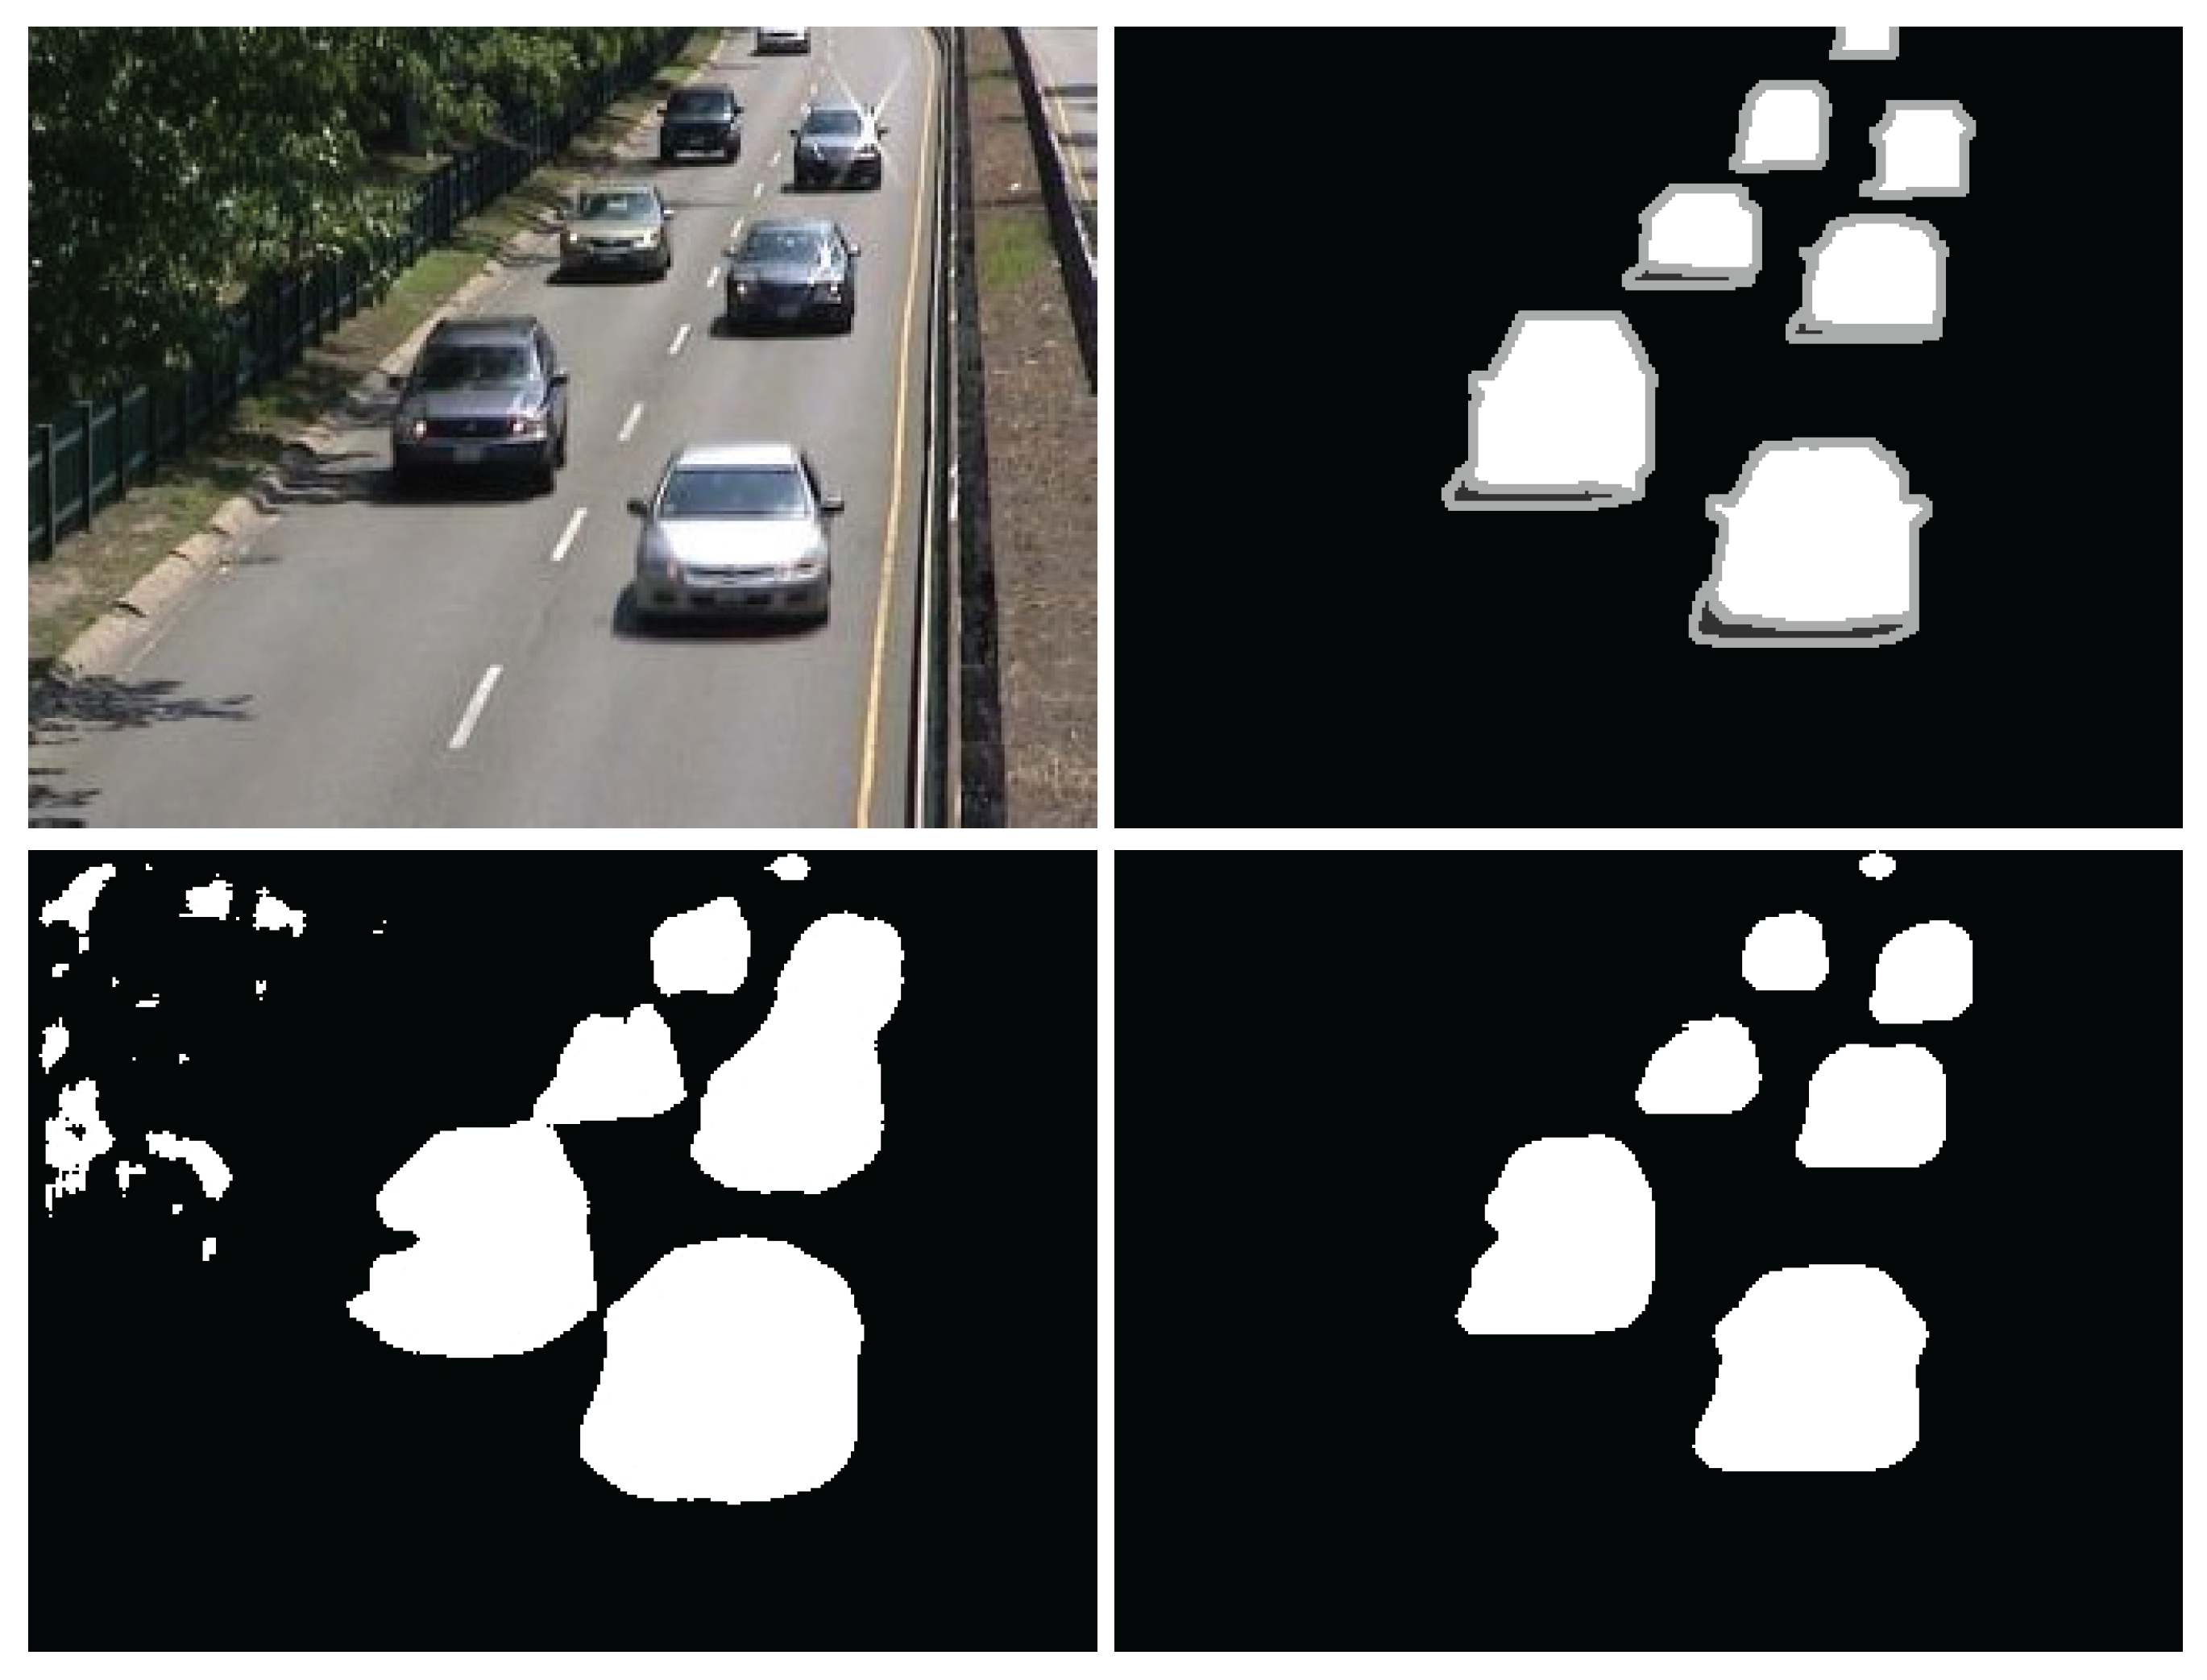
\includegraphics[width=.9\linewidth]{img/chapter2_background/robustBackgroundSubtraction.png}
		\caption{Foreground Detection \cite{Zeng2017}}
	\end{subfigure}%
	\hspace{\fill} 
	\begin{subfigure}[b]{.5\textwidth}
		\centering
		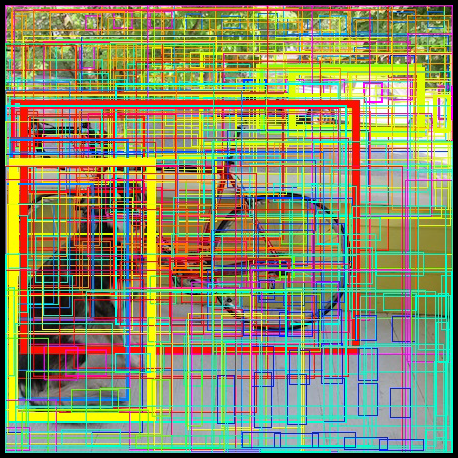
\includegraphics[width=.675\linewidth]{img/chapter2_background/yoloBBBoxes.png}
		\caption{Scanning Window \cite{Redmon}}
	\end{subfigure}
	\vspace{-2\baselineskip}
	\begin{center}
		
		\caption{Comparison of Foreground Detection and Scanning Windows}
		\label{fig:foregroundVsScanning}
	\end{center}
	\vspace{-2\baselineskip}
\end{figure}

\subsubsection{Foreground Detection}
Background subtraction is a widely used approach for detecting moving objects \cite{Piccardi2004}. A temporal average filter can be used to find the median of all the pixels in an image to form a reference image. Frames with moving objects can then be compared pixelwise to the reference, and a threshold set to determines if the pixel is part of the background or foreground. People counting and human detection can then be achieved by segmenting the foreground image into individuals.

\paragraph{} However, this technique often relies on a static camera in a well placed location. This brings up several reasons as to why this method would not be suitable for this project. Firstly, the camera available is part of a head-mounted augmented reality device. The wearer has the ability to move the camera in 6 degrees of freedom. Secondly, the wearer will also be navigating a powered wheelchair. As a result, the background is constantly changing, and the reference image would require constant recomputation before human detection can even begin.

\subsubsection{Scanning Windows}
Due to the ever-changing surroundings of a mobile robot, a better approach for object detection is to exhaustively search an image using scanning windows and determining if an object was detected in each window. However, it must be noted that this method is computationally expensive. In order to achieve real-time detection on a mobile robot, the use of a graphics processing unit (GPU) should be considered \cite{Hirabayashi}.

\subsubsection{Classical Object Detection}

\paragraph{Haar Cascades}
Haar cascades classifies images based on the value of simple features \cite{Viola2001}, which are variants of the difference between the sum of pixel values in rectangular regions. An intermediate representation of the original image is used to rapidly compute a small set of representative rectangular features.

\paragraph{}A cascade of classifiers is then used to determine if the region is detected as a human. The detection process is that of a degenerate decision tree, where a positive result in the first cascade will trigerr an evaluation in the second, more successful classifier. As such, the initial classifier can eliminate a large number of negative examples with very little processing. After several stages, the number of sub-windows has been reduced radically

\paragraph{Histograms of Oriented Gradients}
The method proposed is implemented by dividing the image window into small spatial regions and calculating a local 1-D histogram of gradient directions for all the pixels in the region. The combined local histograms form the overall feature representation of the image.

\paragraph{}The detection window is tiled with the Histogram of Oriented Gradient (HOG) descriptors. In the original paper \cite{Dalal2005}, these feature vectors were then used in a conventional SVM based window classifier  to give human detections.

\subsubsection{Deep Learning Object Detection}
Modern approaches for human detection largely depend on Deep Convolutional Neural Networks (CNN). The approach provides the best in class performance, as well as scaling effectively with more data. An added advantage of using CNN based object detection systems for this project is that they are also capable of detecting multiple classes of objects.

\paragraph{}An issue with CNN approaches is that the methods are trying to draw bounding boxes around objects of interest in images. However, we do not know the number of objects in the image beforehand. As such, to be completely sure every object has been detected, a naive solution is to take a huge number of regions and attempt to classify all the objects in the region, a computationaly expensive process.

\begin{figure}[ht]
	\centering
	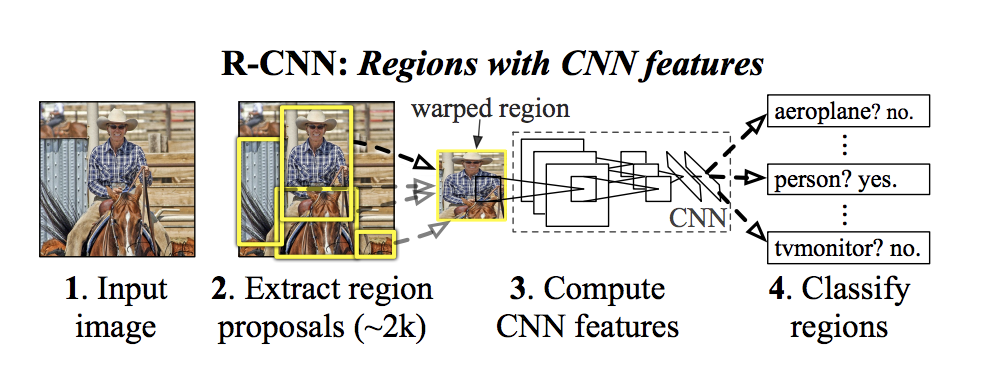
\includegraphics[width=.9\linewidth]{img/chapter2_background/rcnn.png}
	\caption{R-CNN Approach}
\end{figure}

\paragraph{R-CNN} The R-CNN method uses a selective search to extract 2000 regions from an image \cite{Girshick2014}. The regions are selected by generating a large number of candidate regions and using a greedy algorithm to recursively combine similar regions into larger ones. The regions are then fed into a CNN that acts as a feature extractor and the output dense layer consists of the features extracted from the image, which are then fed into an SVM to classify the presence of objects in the region.

\paragraph{}The major disadvantage to this approach is the amount of time required to train the network. Each training image has to be classied once for each of the 2000 region proposals. Furthermore, the selective search algorithm is a fixed algorithm (no learning is done), and as such, could lead to generation of bad candidate region proposals.

\paragraph{YOLO} Whereas R-CNN uses regions to localize the object within an image, You Only Look Once (YOLO) looks at the image as a whole and uses a single CNN to predict the bounding box and the class probabilities \cite{Redmon}. By looking at the image as a whole, the network can use features from the entire image to predict each bounding box.

\begin{figure}[ht]
	\centering
	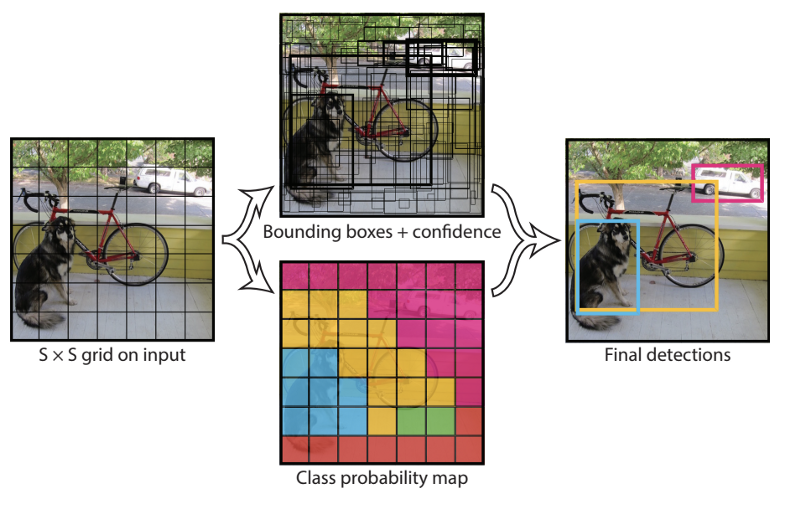
\includegraphics[width=.6\linewidth]{img/chapter2_background/yoloApproach.png}
	\caption{YOLO Approach}
\end{figure}

The model divides the image into an $S \times S$ grid, and for each cell, predicts a number of bounding boxes, the confidence for those boxes and the class probabilities.

\subsection{Comments} \label{sec:detector}
As seen from the research, we can clearly see that there are many ways to solve the human detection problem. The classical approaches, although computationally efficient, are siginficiantly outperformed by the deep learning approaches. For a mobile robot in a public area, we want to be able to detect almost all humans in the surroundings to better inform the PWU.

\paragraph{}However, the major disadvantage of the deep learning approach is the time taken to train the network, as well as the requirement of a GPU to achieve real-time performance. These issues will be addressed in a later section of the report.

\section{Object Tracking}
Object tracking can be defined as the ability to detect objects in consecutive frames and determining if the same objects are present. The techniques are often used in security and surveillance to track individuals across multiple cameras. A more relevant use of object tracking is in augmented reality with ARMarkers to allow for more accurate placements of holograms as the user moves through the AR world.

\subsection{Direction of Research}
 A common scenario for PWU in public spaces is having multiple people walking in the surroundings. Ideally, the augmented reality system should be able to track the same people across frames to be able to determine their direction of motion. As such, we focus our research on the multiple object tracking (MOT) problem in real-time. For an augmented reality system for a PWU, the object tracking must be done in real-time in order to feedback to the PWU. This narrows our field of research to online object tracking techniques.
 
\subsection{Review of Exisiting Methodologies} \label{sec:objectTrack}
 Pedestrian detection is often achieved by using a high quality object detector and associating the detections across frames \cite{Dicle2013}. The associations are based on the appearance and location similarity. Furthermore, it is possible to discern simple motion patterns from the tracked pedestrians, allowing for more accurate tracking.
 
\subsubsection{SORT}
\paragraph{Methodology} The Simple Online and Realtime Tracking (SORT) method relies on the accurate detections of a CNN to calculate bounding boxes of the tracked objects across frames \cite{Bewley2016}. The technique estimates the inter-frame displacements of each detected objects with a linear constant velocity model. The state of each tracked object is modelled using the bounding box centroids $u$ and $v$, the scale and aspect ratio, $s$ and $r$.

\[x = [u, v, s, r, \dot{u}, \dot{v}, \dot{s}] \]

When a new detection is associated with a tracked object, the bounding box of the new detection is used to update the tracked object state, and using a Kalman filter to update the velocity components \cite{Kalman1961}. To determine associations between new detections and tracked targets, the SORT algorithm relies on the intersection-over-union (IOU) distance between each detection and the predicted bounding boxes of all the existing targets.

\paragraph{} For every detection to be tracked, a uniqe tracker identity must be created and destroyed when the object enters and leaves the image. The original implmentation of the algorithm relied on a $IOU_{min}$ value to signify the existence of an untracked object. The tracks are then terminated if they are not detected for an allotted number of frames, to prevent the unbounded growth of trackers.

\paragraph{Limitations}
Due to the simplicity of the association metric, the significant overhead and complexity of object re-identification is removed, allowing for the system to work in real-time applications. However, this also reduces the accuracy of the tracking, since occlusions will spawn new trackers for the same objects. Furthermore, the accuracy of the tracking is largely dependent on the object detector providing accurate bounding boxes.

\subsubsection{Deep SORT}
The original SORT suffered from a high number of identity switches, since the association metric was only accurate if the state estimation uncertainty was low. Wokje proposed a solution to the issue by learning a deep association metric on a re-identification dataset \cite{Wojke2018}. 

\paragraph{Methodology} The tracking and Kalman filtering in Deep SORT is mostly identical to the original SORT implementation. However, Deep SORT uses a Mahalonibis distance as an association metric between the Kalman predicted states and new detections. It further uses a second metric, whereby an appearance descriptor is calculated for each bounding box. A gallery of the previous $L_{k} = 100$ descriptors are kept for each track. The algorithm then iterates and measures the smallest cosine distance between the existing tracks and the detection.

\paragraph{} The appearance descriptor is implemented using a CNN that has been trained offline on a person re-identification dataset. The Github implementation of the Deep SORT algorithm uses a simple nearest neighbour query without any additional metric learning.

\paragraph{Limitations}
Although the accuracy of the the tracking is improved and the issue of occlusions is reduced, the increased complexity of the algorithm requires more computational power. As stated in the paper, a modern GPU would be required to run this in real-time, due to the need for an appearance descriptor to be calculated for each detection.

\subsection{Comments} \label{sec:objectTrackComments}
For this project, we have limited ourselves to researching simple object tracking methods that work in real-time. We can clearly see a trade-off between accuracy of tracking and computational power. Further investigation into the hardware available and the importance of object tracker accuracy will be needed to decide what method would be best for the augmented reality system.

\section{Head and Body Pose Estimation}
Pose estimation is a general computer vision problem where we attempt to detect the position and orientation of an object. This process can be achieved by detecting keypoint locations that describe the pose of the object. For instance, in body pose estimation, we identify the joints in the body.

\subsection{Direction of Research}
An interesting concept to explore is that of head and body pose estimation as a way of infering the direction a person is walking in. For instance, people tend to look in the direction they are currently walking, but should they want to change direction, they also tend to look in that direction before changing \cite{Valenti2012}. Similarly, if we can determine the body pose of a person, the system will be able to tell if a person is walking to or away from the PWU without relying on depth sensors.

\subsection{Review of Existing Methodologies}

\subsubsection{Head Pose Estimation} \label{sec:backHeadPoseEstimation}
Head pose estimation is intrinsically linked with visual gaze estimation \cite{Murphy-Chutorian2009}. If we can characterize the direction and focus of a person's eyes, it may be possible to determine the direction they will walk in next.

\paragraph{Facial Landmark Detection}
Before head pose estimation can be done, keypoints on the face must be detected \cite{Kazemi2014}. These points will then be used to solve a Perspective-n-Point (PnP) problem to determine the head pose. There are many facial landmark detection techniques, depending on the number of landmarks to be detected. As the number of landmarks increase, the more accurate the pose estimation can be. However, it also increases the complexity of the detection, and as such, it becomes a trade-off between the two factors.

\subsubsection{Body Pose Estimation} \label{sec:backBodyPoseEstimation}
An idea we wish to explore is using the body pose of an individual to estimate the direction they are walking in. If the system can discern between a person's back or front, we can infer the motion, since people do not normally walk backwards. A limitation of our system is that it has to be done in real time for it to be effective. As such, the techniques we can explore are limited by the hardware available.

\paragraph{PoseNet} A common approach for body pose estimation is to employ a person detector and perform single-person pose estimation for each detection, known as a top-down approach. PoseNet is a real-time human pose estimator with a web-browser implementation that runs on Tensorflow.js, making it easily available to anyone. The implementation is based on the works of Papanderou and Zhu \cite{Papandreou2017} in building a network that utilizes the Faster-RCNN model as an object detector to obtain accurate bounding boxes of people in an image \cite{Ren2017}. The keypoints are then calculated using a a ResNet \cite{He2016} by predicting activation heatmaps and offsets.

\paragraph{OpenPose} Top-down approaches can be limited by the failure of the person detector. This is especially common when two individuals are very close to each other, and the detector is unable to differentiate between them. In contrast the bottom-up approach, which is based on partitioning and labeling an initial pool of body part candidates into subsets \cite{Pishchulin}, is able to deal with an unknown number of people, and can infer that number by linking the part hypotheses.

\begin{figure}[ht]
	\centering
	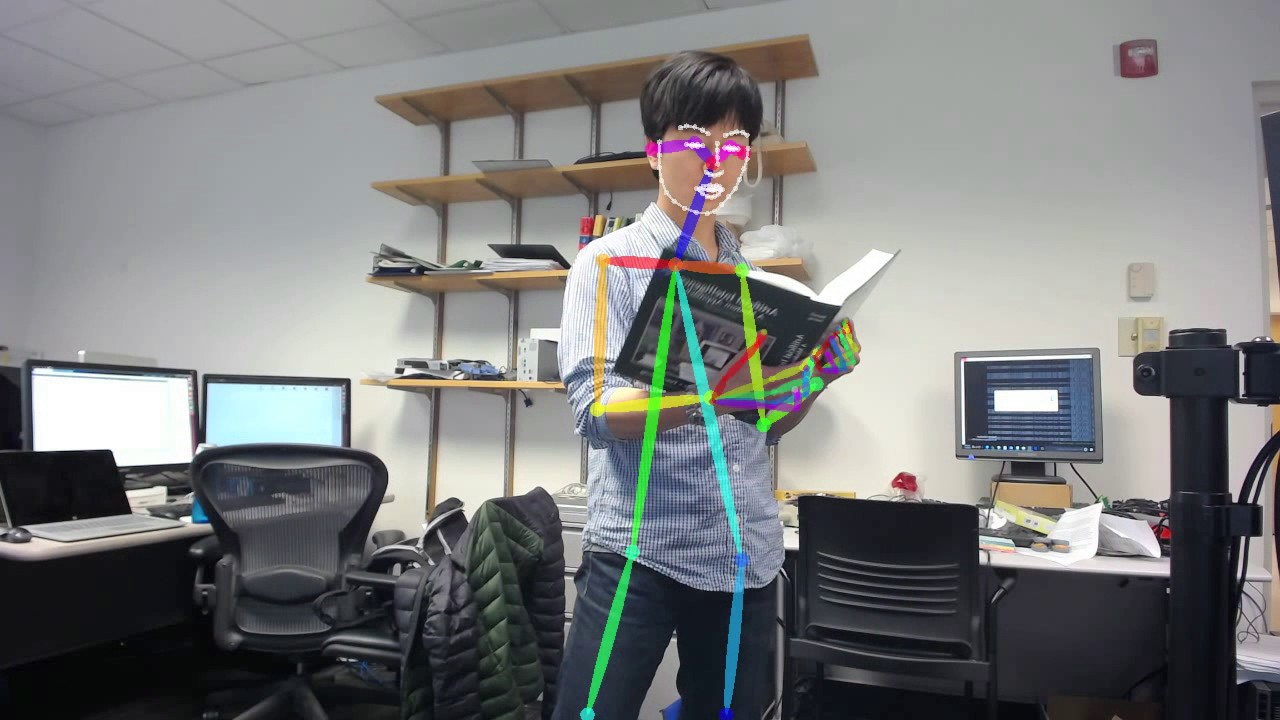
\includegraphics[width=.7\linewidth]{img/chapter2_background/openpose.jpg}
	\caption{OpenPose body pose detection \cite{Cao2017}}
\end{figure}

\paragraph{} As such, OpenPose presents a method of multi-person pose esimtation using a bottom-up approach \cite{Cao2017}. The method relies on \textit{partial affinity fields} (PAFs), a representation that encodes unstructured pairwise relationships between body parts. The network produces the 2D confidence maps of body part locations and PAFs, and through greedy inference, the network outputs the 2D keypoints for all people in the image.

\subsection{Comments}
Head and body pose estimation is a vast field of research, with dozens of effective real-time estimation methods. This project is not focused on achieving the best body/head pose estimation, but rather, in utilizing existing frameworks to infer directions of individuals. As such, we have refrained from delving too deep into the theory of body pose estimation, and instead, have attempted to choose a method from available implementations.

\section{SLAM}
The term mapping refers to a system that will create a map of the surrounding areas, by detecting objects such as walls and other obstacles. In order to help users navigate, the system must analyse the surroundings for potential dangers. As such, it is important to build up a thorough and complete map.

\paragraph{}A fundamental method for robot navigation is the Simultaneous Localization And Mapping (SLAM) method. The process allows the system to predict the trajectory of the robot and the location of all objects on-line, without the need of an \textit{a priori} knowledge of the robots location \citep{Bailey2006a}. The method estimates the pose of the robot relative to landmarks which are detected. The popularity of SLAM increased with the emergence of indoor applications of robotic devices.

\subsection{Direction of Research}
For a PWU to navigate a wheelchair effectively through public spaces, they need to be able to avoid colliding with people or obstacles. An accurate map of the surroundings is key to solving this issue. However, some techniques rely on pre-existing maps of the area. A PWU may navigate their wheelchair to new locations, and can not rely on pre-existing maps for accurate navigation. Rather, the goal is to build up a real-time map of the surroundings that is accurate enough to avoid collisions.

\subsection{Review of Existing Methodologies}
A review of SLAM techniques can be found in \cite{Cadena2016}, which also outlines the standard formulation of the SLAM problem as that of a Maximum a posteriori (MAP) estimation. The formulation relies on Bayes theorem, and using the prior knowledge of the robots pose to maximize the likelihood to estimate the current position of the robot. The variables required to estimate the position are the robot poses, the position of landmarks and the calibration parameters of the sensors.

\paragraph{}In order to build an accurate map of the surroundings, the calibration of the sensors providing the measurements is a crucial step. The choice of sensors also matter, as the type of data returned by the sensor may affect the computational complexity of the SLAM algorithm. As such, it is common to have a module in the system that deals with the extraction of relevant features from the sensor data.

\paragraph{}A fairly common assumption in SLAM approaches is that the world is static and remains unchanged as the robot moves. This becomes an issue with the goal of this project, which hopes to achieve the ability to detect human objects walking around the wheelchair. This issue will be addressed in a later section.

\subsubsection{Visual SLAM}
Visual SLAM (vSLAM) is an implementation of SLAM that relies on visual inputs only. As stated in \cite{Taketomi2017}, vSLAM is suitable for AR due to the low computational algorithms that can be implemented on the limited resources of an AR headset. The technique of vSlam is mainly composed of three modules:

\paragraph{Initialization}
In the initialization stage, camera pose estimation is conducted, to transform objects in a 2D image from the camera into a 3D co-ordinate system that the robot understands. This process determines the position and orientation of the camera relative to the object. A part of the environment is reconstructed as part of the initial map using the global co-ordinate system of the robot.

\paragraph{Tracking}
Here, the reconstructed map is used to estimate the pose of the camera with respect to the map. Feature mapping or feature tracking is conducted on the images in order to get a 2D-3D correspondence between the image and the map. The camera pose can then be calculated from the correspondences by solving the Perspective-n-Point problem \citep{Nister2004}. This allows the system to identify where on the map the robot currently is.

\paragraph{Mapping}
When the robot passes through an environment that has previously not been mapped, the 3D structure of the surroundings is calculated from the camera images. The structures are then added to the existing map of the environment.

\subsection{Comments}
Due to the freedom in movement of an augmented reality headset camera, a system that relies solely on visual inputs may not be able to detect all obstacles in the surroundings. For instance, a limitation is that the PWU will not be able to extend their head backwards to view objects behind them. As such, it becomes important to consider the sensors available on powered wheelchairs, and utilize them to build an accurate map of the surroundings.

\section{Augmented Reality Headsets}
The improvements in augmented reality technology has spurred research into the use of AR devices in everyday tasks. The availability of commercial devices has also encouraged developments in the field, with products such as the Microsoft Hololens and the Magic Leap One.

\subsection{Direction of Research}
The augmented reality system built for this project needs to be able to give visual prompts to the PWU. As such, a device that already has the ability to create holograms is key. Furthermore, most AR devices have built in cameras to perceive the world around the user. We hope to be able to access the cameras on the device to do object detection and tracking.

\subsection{Review of Existing Methods}

\subsubsection{Microsoft Hololens}
The Microsoft Hololens is an untethered holographic computer, allowing for the display of 3D holograms pinned to real world objects. The Hololens is equipped with an array of sensors, making it an ideal choice of hardware for this project.

\paragraph{Holograms}The Microsoft Hololens is able to blend real world and virtual content into environments where digital and physical objects can co-exist and interact. The term 'Mixed Reality' was first introduced by \cite{Milgram1994}, and refers to the blending of the physical and virtual worlds.

\paragraph{}The Hololens allows the developer to create 'Holograms', which are objects of light and sound that are displayed by the headset. Users are able to interact with the holograms through voice, gaze and gestures. Enhanced environment apps are applications that facilitate the placement of digital information on the user's current environment \citep{Microsofta}. An example of an enhanced environment application is placing markers in augmented reality on objects that the user can interact with in both the physical and digital worlds. 

\paragraph{Hardware Specifications} As part of our research, we highlight the sensors on the device that may be relevant to the project. A full hardware specification is available online \cite{Microsoft2015}. 

\begin{itemize}
	\item 1 Intertial Measurement Unit (IMU)
	\item 4 Environment understanding cameras
	\item 1 Depth Camera
	\item 1 2MP Photo/HD video camera
\end{itemize}

\paragraph{} Most importantly, the Hololens has a video camera. Preliminary research shows that it is possible to access the camera data directly, making it a suitable choice for the project.

\paragraph{Personal Robotics Lab} The use of augmented reality devices to help PWUs is a research topic actively pursued by members of the Personal Robotics Lab at Imperial College London. Previous work has explored the use of augmented reality as a visualization tool to help PWUs understand the system dynamics of the wheelchair they operate, displaying visual cues that indicate the direction of travel of assistive control \cite{Zolotas2018}. Other work involves using the camera to detect objects of interest in the environment, and developing a system that navigates the wheelchair to the detected objects through gaze and eye tracking \cite{Chacon-Quesada}.

\begin{figure}[ht]
	\centering
	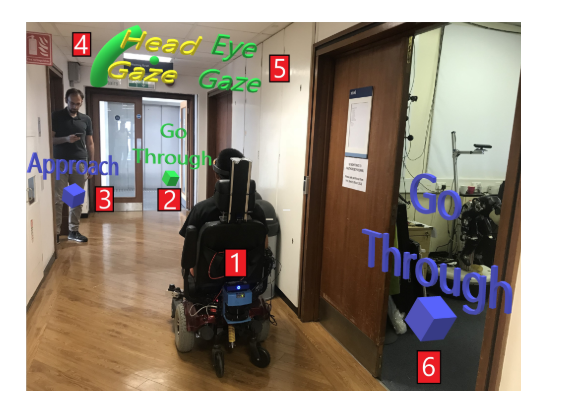
\includegraphics[width=.5\linewidth]{img/chapter2_background/AR_Interface.png}
	\caption{AR visualizations and markers for interaction \cite{Chacon-Quesada}}
\end{figure}

\subsection{Comments}
Although other AR-devices exist on the market, due to the availability of the Microsoft Hololens in the Personal Robotics Lab, as well as the research done by individuals, it is in the best interests of this project to use the Hololens as the main augmented reality device for this project.

\chapter{Requirements Capture}

\section{Project Deliverable}
The objective of this project is to develop an augmented reality system that can be used by powered wheelchair users (PWUs) to assist them in navigating their powered wheelchairs in public spaces with many people walking in the surroundings. The system should be able to detect the presence of individuals and infer their position relative to the PWU, and by extensions, estimate their direction of travel.

\paragraph{}We propose a system that uses the Microsoft Hololens augmented reality headset as the main input and visualization tool. The PWU would wear the headset as they operate the powered wheelchair, allowing the system to create visualizations of potential obstacles and collisions. Furthermore, the system would also encompasses the reactive control aspect of the powered wheelchair. Should an individual be detected as walking in the wheelchairs trajectory, the system will send control signals to the powered wheelchair to slow down or completely stop depending on how far the target is from the wheelchair.

\paragraph{} By definition of the requirements, we can divide the project into three parts: Human Detection and Direction, Obstacle Mapping \& Visualization, and finally Reactive Control.

\section{Human Detection and Direction}
The requirements of the Human Detection and Direction (HDD) system is to be able to use a video stream of the surroundings to determine the position and direction of people. The Hololens has a built in camera that can be used to take photos of the surroundings of the user \cite{Chacon-Quesada}. We will leverage this ability to create a video stream.

\paragraph{}The actual HDD system is implemented on another computer with access to a GPU. We utilize the GPU to be able to do real-time object detection and pose estimation of detected individuals. The system should be able to infer the direction individuals are walking in, as well as their real-world positions relative to the PWU.

\paragraph{Features} 
\begin{itemize}
	\item Creating a live video stream using camera.
	\item Streaming the live video to accompanying computer.
	\item Object detector trained on humans/pedestrians.
	\item Object tracker to track detected humans, and determine their direction.
	\item Body/Head pose estimator to determine direction of travel.
	\item Stream detections back to the Hololens for visualization.
\end{itemize}

\section{Obstacle Mapping \& Visualization }
This project utilizes the Microsoft Hololens as a visualization and spatial mapping tool. The HDD system will output its detections and directions to the Hololens, which is used to create visualizations that will help the PWU. Examples of the visualization include arrows that indicate direction of movement, as well as alerting the user to potential collisions.

\paragraph{Features}
\begin{itemize}
	\item Receiving detection/direction data from HDD system.
	\item Utilize Camera to World transforms of the Hololens Camera to get World co-ordinates of people.
	\item Create holographic visualizations to help PWU understand the direction people are walking in.
	\item Create a map of obstacles for Reactive Control.
\end{itemize}
 
\section{Reactive Control} \label{sec:reactive}
The powered wheelchair (ARTA) available in the Personal Robotics Lab (PRL) can be manually operated using a joystick. The goal of the project is for the PWU to be able to wear the Hololens as an aid for navigation in public spaces. As such, it would be beneficial for the PWU if the wheelchair had the ability to reactively control the device to prevent collisions with detected objects.

\paragraph{Features}
\begin{itemize}
	\item Receiving object detections in front of wheelchair.
	\item Prevent wheelchairs from driving into objects.
\end{itemize}

\chapter{Analysis and Design} \label{chapter:4}
This chapter gives an overview of the overall system and explains the design choices made. Throughout the project, we explored various methods to implement a real-time augmented reality system for PWUs operating a wheelchair. Naturally, the structure and goals of the project have developed since the interim report, and we review the differences between the initial goals and final product .

\section{Design Overview}
As stated in the requirements, this project consists of three major components:
\begin{itemize}
	\item Human Detection and Direction (HDD)
	\item Object Mapping and Visualization (OMV)
	\item Reactive Control on ARTA
\end{itemize}

\begin{figure}[ht]
	\centering
	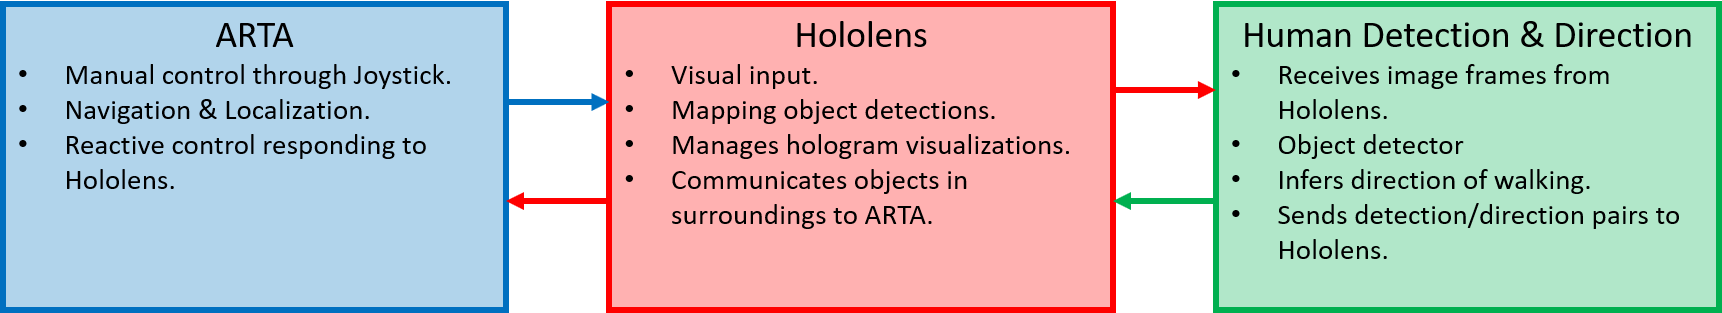
\includegraphics[width=1.0\linewidth]{img/chapter4_analysis/simpleSystemDiagram.png}
	\caption{Simplified high level system diagram}
	\label{fig:simplifiedHL}
\end{figure}

From a very high level view, we can map these requirements to the respective devices they will be operating on. The HDD system takes implements the object detection and human direction inference, while the Hololens is responsible for utilizing the spatial mapping to obtain world positions of the detections, as well as visualizing the detections. The powered wheelchair (ARTA), has manual input that is overridden by the reactive control system that is dependent upon the detections and mappings. The diagram in Figure. \ref{fig:simplifiedHL} shows an overview of the system, and shows that the Hololens acts as an intermediary between ARTA and the HDD.

\subsection{Hardware}

\begin{table}[ht]
	\centering
	\begin{tabular}{l|l|l|l|}
		\cline{2-4}
		& \multicolumn{1}{c|}{\textbf{ARTA}}                                                 & \multicolumn{1}{c|}{\textbf{Hololens}} & \multicolumn{1}{c|}{\textbf{HDD}}                              \\ \hline
		\multicolumn{1}{|l|}{\textbf{Hardware}}         & \begin{tabular}[c]{@{}l@{}}Powered Wheelchair \\ controlled by Laptop\end{tabular} & Hololens                               & \begin{tabular}[c]{@{}l@{}}Desktop PC \\ with GPU\end{tabular} \\ \hline
		\multicolumn{1}{|l|}{\textbf{Operating System}} & Ubuntu 16.04                                                                       & UWP                                    & Ubuntu 16.04                                                   \\ \hline
	\end{tabular}
	\caption{Hardware description of system}
	\label{tab:hardware}
\end{table}

Table. \ref{tab:hardware} summarises the hardware overall system is implemented on. The powered wheelchair, ARTA, is controlled by a laptop, which is responsible for the wheelchair speed, wheel rotations, navigation and localisation. The Hololens is a self contained augmented reality headset, running the Universal Windows Platform (UWP) operating system. Finally, the Human Detection \& Direction system is implemented on a desktop computer with a GTX 1050Ti GPU, allowing it to run real time object detectors.

\subsection{System Communication} \label{sec:systemComms}

\subsubsection{Robotic Operating System} Since the project spans multiple operating systems, we have chosen to utilize the Robotic Operating System (ROS) as a means of communication between the devices. In ROS, a \textit{node} is defined as a process that performs a computation. A node can be made up of smaller nodes that perform specific computations that serve the needs of the parent node. We can think of the three major systems as large ROS nodes that consists of smaller nodes that run individiual tasks, such as creating the camera stream, or detecting objects.

\paragraph{ROS Topics} Nodes in ROS communicate with one another by publishing data in the form of \textit{messages} which get broadcasted over a \textit{topic}. Nodes can choose what data they receive by subscribing to topics. This method allows for nodes running on different devices to communicate with each other, regardless of the operating system. The nodes are unaware that the data it receives is published from a node running on a seperate computer, making ROS a perfect choice for communication in this design.

\section{Human Detection \& Direction System}
The HDD system is reponsible for detecting and predicting the directions of people in the surroundings of the wheelchair. By taking visual inputs in the form of images from the Hololens, we run an object detector trained on a dataset of pedestrians to detect people and heads. The bounding boxes produced by the object detector are fed as inputs to an object tracker and a body pose estimator. We use the results of these two nodes to infer the direction a detected person is moving in, and publish the results back to the Hololens.


We present an overall view of the HDD System, covering the purpose and design of individual components. We also propose the reasoning behind certain design choices, which we cover in more depth later in this report.

\subsection{YOLO Object Detector} \label{sec:yolo}
Object detectors often form the input to an object tracker or pose estimation system \cite{Bewley2016, Jin2017}. In the case of top-down body pose estimation methods, detections can be the first point of failure \cite{Insafutdinov}. As such, the accuracy of the chosen object detector must be considered, together with the choice of using a pre-trained model or training on a more relevant dataset. Finally, we must also consider the use-case of the detector, which must be able to operate in real-time and detect moving objects as they pass by.

\subsubsection{Choice of Detector}
As commented on in Section \ref{sec:detector}, modern deep learning techniques outperform classical object detectors in accuracy, but are limited by the requirement of a GPU to perform in real-time. Since the Hololens does not have built in support to run object detection networks, Microsoft provides the Azure Cognitive Services API to allow developers to query their system for object detections. The limitation is that this service is not free, and abstracts away the implementation of an object detector. Furthermore, one of the personal goals for this project was to learn more about CNNs in computer vision.

\paragraph{} Taking this into account, we compared several deep learning architectures for object detection. Previous work done in the PRL used Facebook AI Research's (FAIR) Detectron to detect objects \cite{Chacon-Quesada, Detectron2018, Rena}. Further discussions with members of the Imperial Computer Vision \& Learning Lab suggested the use of the YOLO object detector \cite{Redmon}, due to its speed and having a lightweight implementation that could be run on lower end GPUS at relatively high frame rates. This prompted the design decision to use the Darknet framework to use the \textbf{YOLOv3-tiny} architecture as the object detection method of choice for this project \cite{Redmon2018}.

\subsubsection{Pre-trained Model vs Training} \label{sec:designYOLO}
An advantage of using the YOLO Darknet framework is that it provides trained models which can detect multiple object classes, including the class \textit{Person}. One of the pre-trained models is the YOLOv3-tiny architecture trained on the Common Objects in Context (COCO) dataset \cite{Lin}.

\paragraph{Comparing Models} To compare the accuracy of the bounding boxes produced by pre-trained model, sample videos were recorded using the Hololens and used as a base comparison point. It was quickly shown that although the COCO trained model can detect individuals, or multiple people who are well spaced out, it had difficulty in differentiating between people who are close together or slighlty occluded. Figure \ref{fig:yoloCHvsCoco} highlights the issue of the COCO model failing to detect small people close together.

\begin{figure}[ht]
	\begin{subfigure}[b]{.5\textwidth}
		\centering
		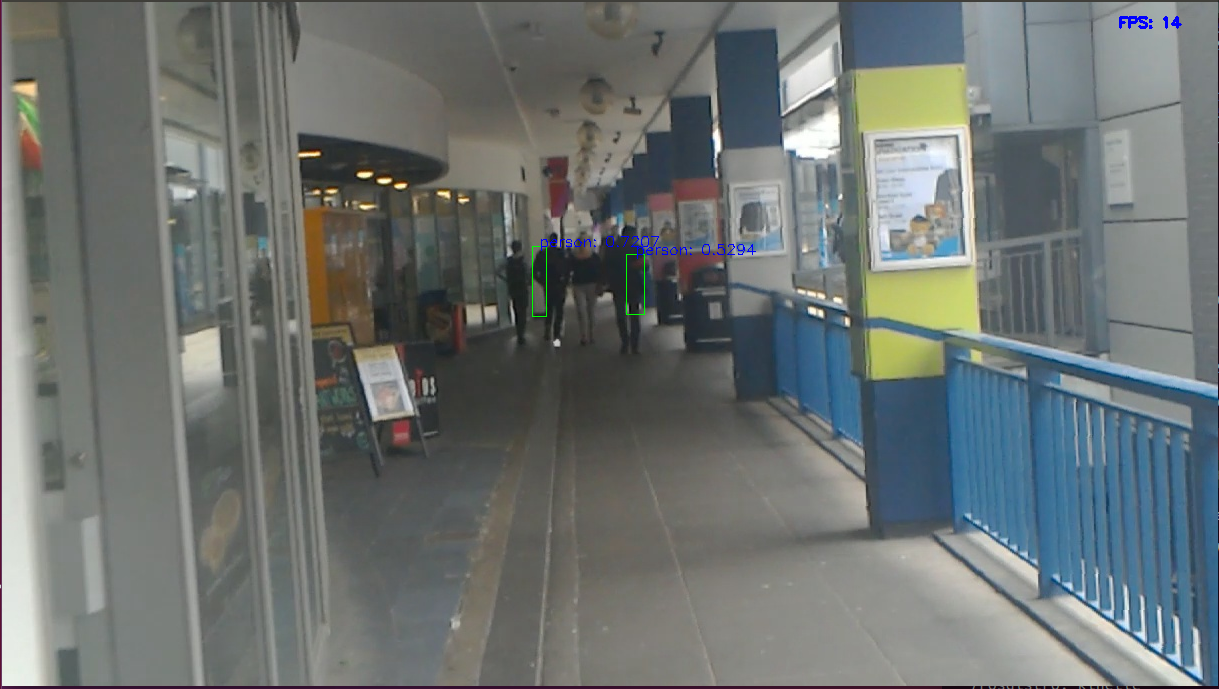
\includegraphics[width=0.95\linewidth]{img/chapter4_analysis/yoloCoco.png}
		\caption{COCO YOLOv3-tiny}
	\end{subfigure}%
	\hspace{\fill} 
	\begin{subfigure}[b]{.5\textwidth}
		\centering
		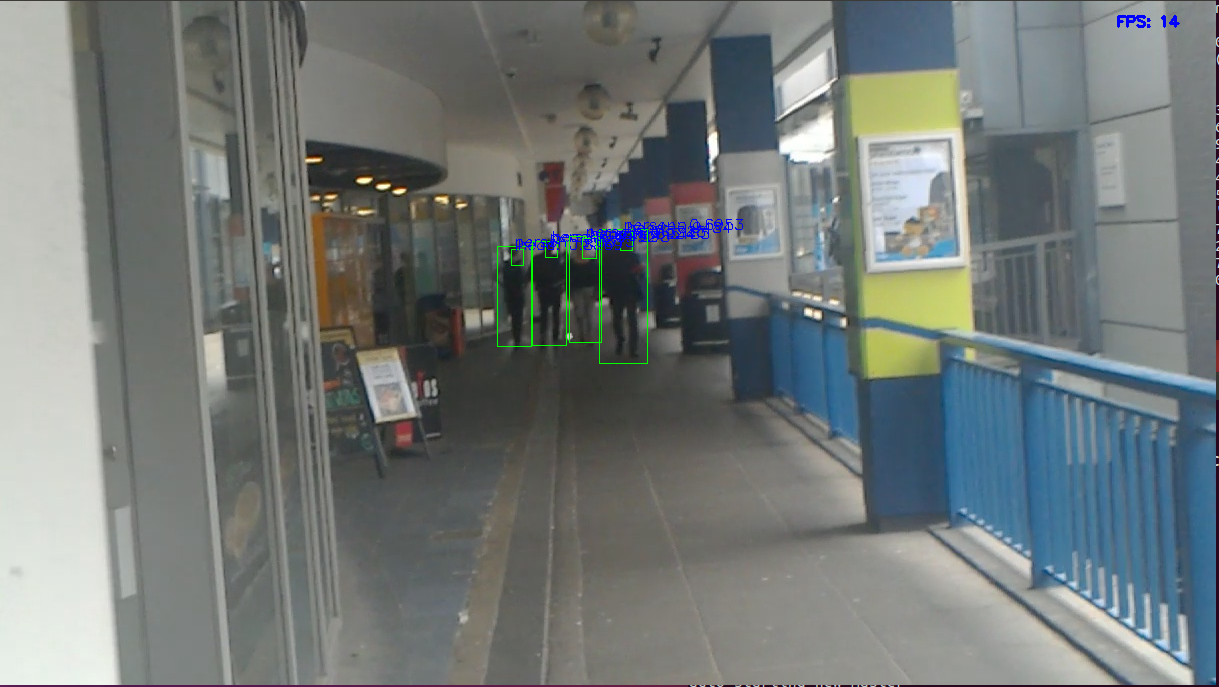
\includegraphics[width=0.95\linewidth]{img/chapter4_analysis/yoloCH.png}
		\caption{Trained YOLOv3-tiny}
	\end{subfigure}
	\vspace{-2\baselineskip}
	\begin{center}
		\caption{Model comparison on a video from Sherfield Walkway at Imperial College London}
		\label{fig:yoloCHvsCoco}
	\end{center}
	\vspace{-2\baselineskip}
\end{figure}

\paragraph{Pedestrian Dataset} A common case in pedestrian detection is occlusion, where only certain parts of an individual are visible.  To resolve this issue, we decided to train the YOLOv3-tiny model on the \textbf{CrowdHuman} dataset \cite{Shao}, which contains annotated images of people in crowded places. The annotations include bounding boxes for the head, visible human region and full-body region. The annotations for partially visible people allows the network to learn to recognize occlusions, reducing the issue of failed detections when people are too close to each other. We also trained the network to detect heads, since we initially wanted to use head pose estimation to determine direction.

\paragraph{Analysis}
The result of training the YOLOv3-tiny model on the CrowdHuman dataset is that the system is able to better detect smaller figures with obscured bodyparts. The additional ability to detect heads allowed us to explore the use of head pose estimation for direction inference. We go into further detail on the training process in the Implementation section of this report.

\subsection{YACHT: Yet Another Crowd Human Tracker}
The bounding boxes produced by the object detector are consumed by the \textbf{Yet Another Crowd Human Tracker} (YACHT) module, which is made up of two nodes. The tracker node uses the Deep SORT algorithm to track detected individuals \cite{Wojke2018}, while the pose estimator node uses the OpenPose \cite{Cao2017} network to determine whether a person is walking towards or away from the PWU.

\paragraph{}In the following sections, we briefly explain the  methods used to infer the directions people are walking in. We also explore the use of head pose estimation, and the limitations that prevented it from making it to the final design.

\subsubsection{YACHT Tracker: Object Tracking}
We explored existing object tracking methods in Section \ref{sec:objectTrack} and discussed our choices in \ref{sec:objectTrackComments}. For moving object tracking on a powered wheelchair, we express the need for an online object tracking system. As such, we chose to investigate two related real-time methods, SORT \cite{Bewley2016} and Deep SORT \cite{Wojke2018}.

\paragraph{SORT}  The Simple Online and Realtime Tracking (SORT) method is a fast online object tracker. The initial implementation of YACHT used the SORT algorithm due to its speed. However, it was quickly realized that due to the simplicity of the association metric, object tracking was not very accurate, especially for occluded objects. When two objects crossed paths, the tracker was unable to recognize the act, and re-labeled the objects with brand new tracking IDs.

\paragraph{Deep SORT} Deep SORT is an extension of the original SORT algorithm, but uses a deep network to generate feature descriptors for the predicted bounding boxes. We explain the algorithm in Section \ref{sec:objectTrack}, but to repeat, instead of using the Intersection-over-Union association metric to compare bounding boxes, the deep network genereates feature descriptors for the bounding box, and a Neareast-Neighbours is used to compare the features with a library of feature vectors for each tracked object. This is a form of person re-identification, and this additional step reduced the problem of trackers being lost due to occlusion.

\begin{figure}[ht]
	\centering
	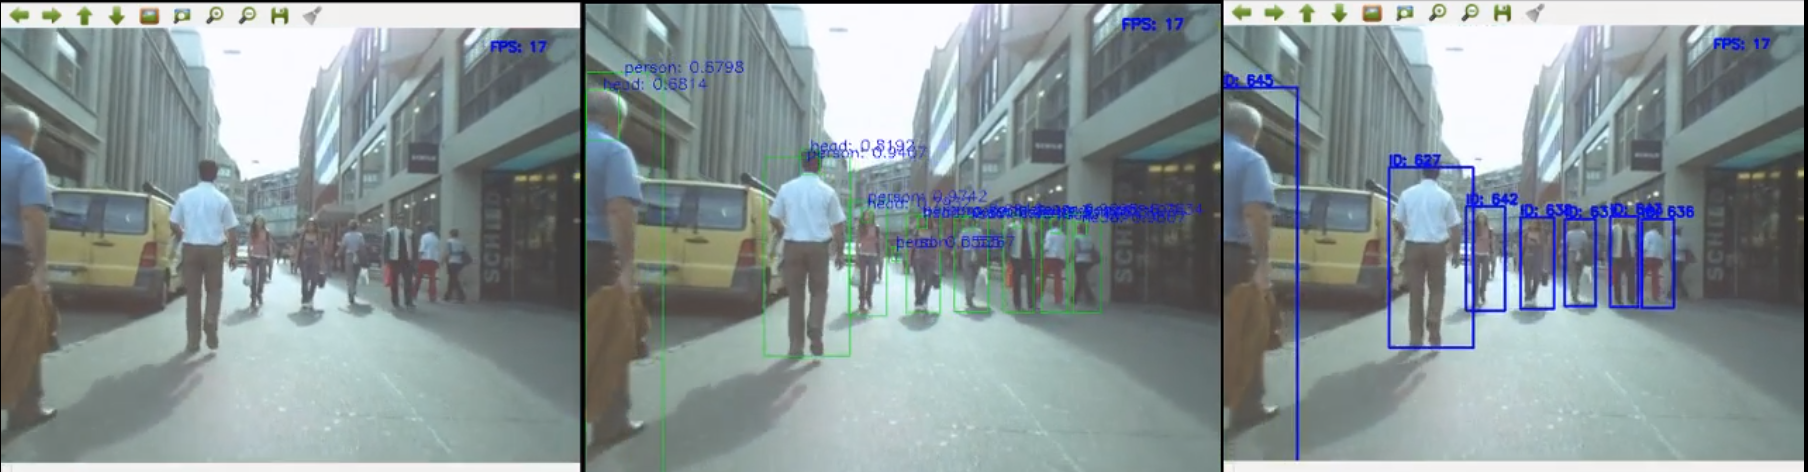
\includegraphics[width=1.0\linewidth]{img/chapter4_analysis/deepSortMOT.png}
	\caption{MOT16 benchmark \cite{Milan} (L) using our YOLO model (M) for Deep SORT (R)}
	\label{fig:deepSortMOT}
	\vspace{-1\baselineskip}
\end{figure}

\paragraph{Analysis} The generation and storage of feature descriptors for tracks is an expensive process. For the system to run in real-time, a GPU is needed to accelerate the network. We have made changes to the Deep SORT implementation so it can run on Tensorflow-GPU, which we explain later in this report. This improves the speed significantly, but uses up precious memory. As a result, we had to consider the amount of memory avaiable on the GPU, since the YOLO detector and OpenPose networks also rely on GPU acceleration. After testing, we found that it was possible to run both networks on the GPU at the same time, and we chose to use the Deep Sort method.

\newpage
\subsubsection{Object Tracking for Direction Inference} \label{sec:objecTrackingDirection}
An idea we explored was to use the previous image co-ordinates of a tracker to predict the direction a person will walk in. This involved storing the previous states of each track and extrapolating the centroids of each track to determine a direction.

\begin{figure}[ht]
	\begin{subfigure}[b]{.45\textwidth}
		\centering
		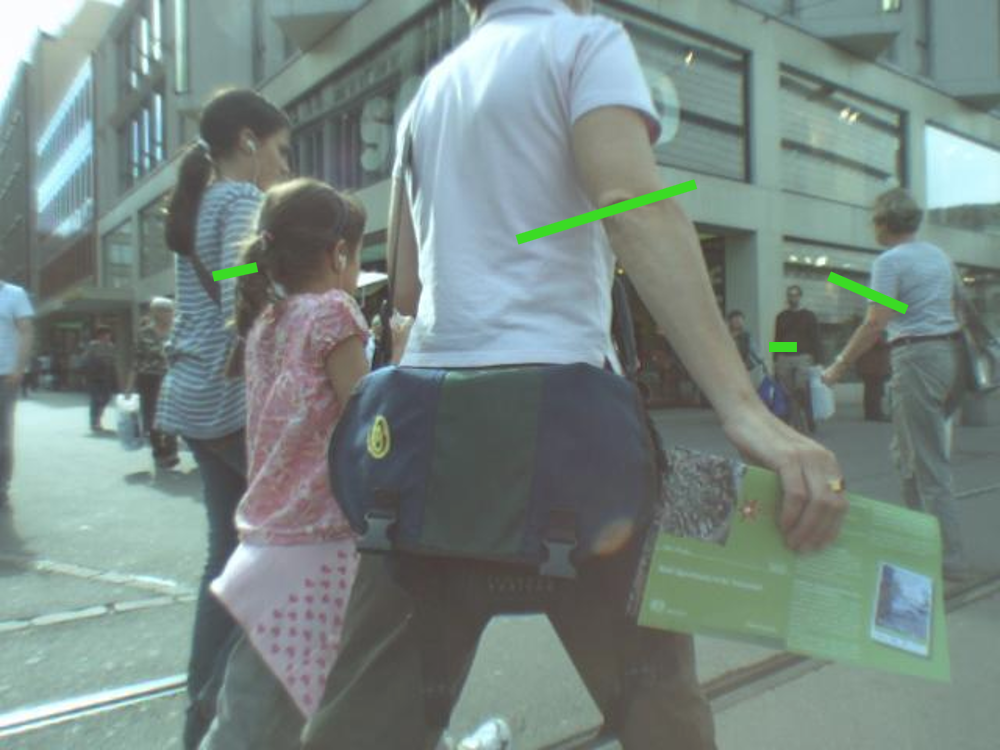
\includegraphics[width=1.0\linewidth]{img/chapter4_analysis/linExDirection.png}
		\caption{Tracks with horizontal motion}
	\end{subfigure}%
	\hspace{\fill} 
	\begin{subfigure}[b]{.45\textwidth}
		\centering
		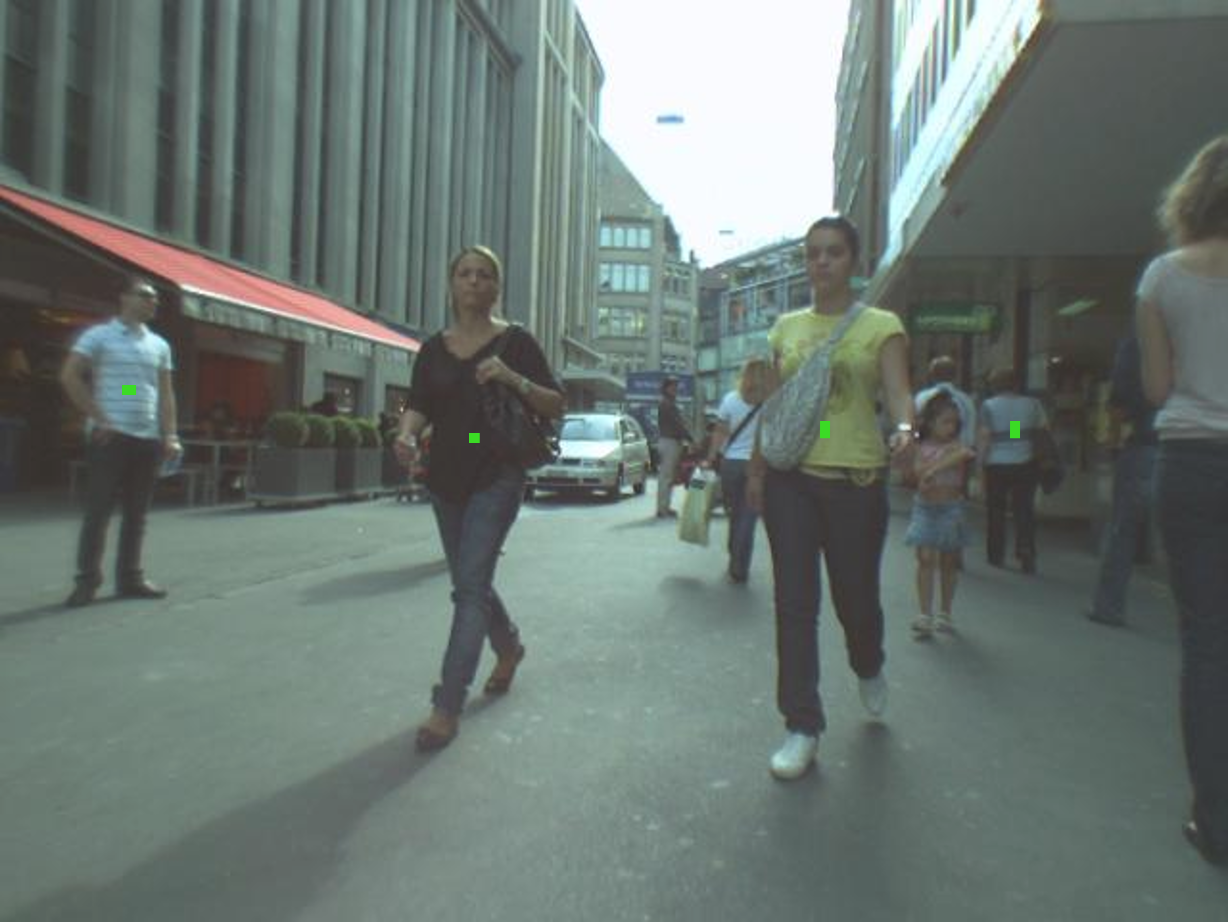
\includegraphics[width=1.0\linewidth]{img/chapter4_analysis/linExDirectionAmb.png}
		\caption{Tracks with mostly vertical motion}
	\end{subfigure}
	\vspace{-1\baselineskip}
	\begin{center}
		\caption{Linear extrapolation works for objects that move across the frame, but it becomes difficult to determine the direction when mostly vertical motion occurs}
		\label{fig:linExProblem}
	\end{center}
	\vspace{-2\baselineskip}
\end{figure}

\paragraph{Algorithm} For each tracked object in a frame:

\begin{algorithm}[ht] 
	\KwData{(x,y) centroid image co-ordinates up to the previous 5 states}
	\KwResult{(x,y) of extrapolated point}
	
	\For{Frame}
	{
		\For{Tracker}
		{
			\If{Tracker existed in previous frame}
			{
				Extrapolate over the centroids of previous states; \\
				Return linear extrapolation (x,y);
			}
			\If{Tracker has no previous states}
			{
				Add (x,y) centroid of tracker to queue of previous states;	\\
				Return current centroid (x,y);
			}
		}
	
	}
\end{algorithm}

\paragraph{Issues} Although the method works for trackers which cover large distances across the frame, linear extrapolation of image co-ordinates suffers when the tracked centroid does not have much horizontal motion. As such, this leads to an ambigious definition of the direction. Since the object is not moving across the screen, it is not possible to differentiate between a person standing still, moving directly towards the PWU or walking away.

\begin{figure}[ht]
	\centering
	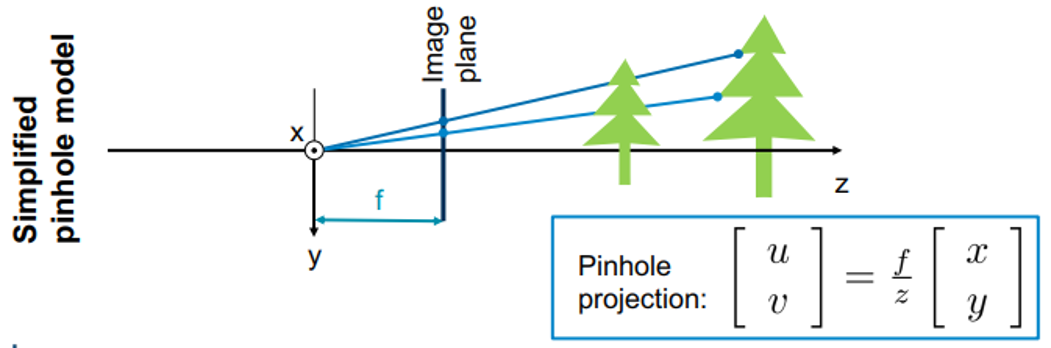
\includegraphics[width=0.8\linewidth]{img/chapter4_analysis/pinholecamera.png}
	\caption{Pinhole Camera projection and the loss of the z-axis \cite{Leutenegger2019}}
	\label{fig:pinhole}
	\vspace{-1\baselineskip}
\end{figure}

\paragraph{} In the pinhole camera model, when an object in the real world is projected onto a 2D image, we lose the distance along the z-axis. The issue of a world-to-camera image projection occurs when we want to obtain the world co-ordinate of an object from the image. Due to the loss of z-axis information, the best we can do is to calculate a ray through the 2D image point. However, as shown in Figure \ref{fig:pinhole}, it becomes impossible to tell how far away the object is without a depth camera, since the object can exist anywhere along that ray.

\subsubsection{YACHT Direction: Body Pose Estimation}
To solve the direction ambiguity brought up in Section \ref{sec:objecTrackingDirection}, we proposed the use of body pose estimation techniques to determine whether a person is walking towards or away from the camera of the PWU. We researched several body pose implementations in Section \ref{sec:backBodyPoseEstimation}, but we ultimately decided on OpenPose, due to its well documented implementation on Github \cite{Cao2017}.

\paragraph{Object Detectors \& Bottom-Up Approaches} The YOLO object detector outputs the original image and the associated bounding box co-ordinates of detections. The OpenPose node consumes the image and performs body pose estimation on the whole image, before matching poses with the object detections. Since OpenPose is a bottom-up approach, we admit that it is counter-intuitive to use an object detector to detect individual people when OpenPose determines the body part keypoints across the whole image. This will be explored more in the evaluation of the report.

\paragraph{Keypoint Estimation}
The OpenPose framework provides several pre-trained models for body pose keypoint estimation. From our tests, we found that the \textit{BODY\_25} model was the fastest, suiting our real-time requirements. Figure \ref{fig:bodyKeyPoints} shows the keypoints generated by the model.

\begin{figure}[ht]
	\centering
	\includegraphics[width=0.2\linewidth]{img/chapter4_analysis/keypoints_pose_25.png}
	\caption{Keypoints produced by the BODY\_25 model \cite{Cao2017}}
	\label{fig:bodyKeyPoints}
\end{figure}

The model identifies 25 keypoints on the human body, and can differentiate between the left and right limbs on the human body. This makes the model suitable for determining if a person is facing the camera or not. We further explain the methodology in the implementation section of the report. From this, the node outputs the direction of the object to the Hololens.

\subsubsection{Head Pose Estimation}
We initially began the project by exploring the use of head-gaze estimation as a novel way of infering the intended direction of motion of a person. We researched the concept of head pose estimation in Section \ref{sec:backHeadPoseEstimation}, with the logic being people tend to look in the direction where they are walking. We leveraged the use of the DeepGaze library as an initial starting point \cite{Patacchiola2017a}, since the library has a built in head-pose estimator. 

\begin{figure}[ht]
	\centering
	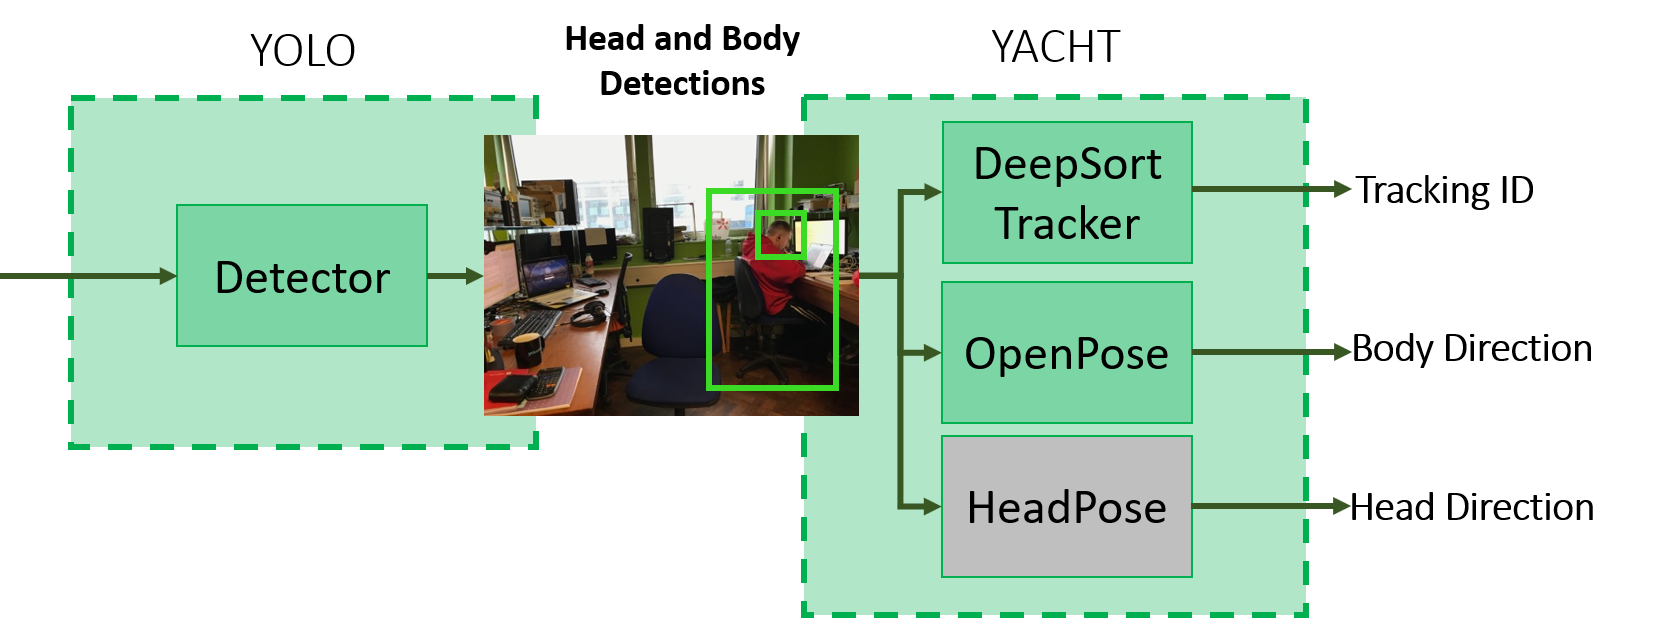
\includegraphics[width=1.0\linewidth]{img/chapter4_analysis/hddSystemHeadPose.png}
	\caption{Initial HDD System with HeadPose}
	\label{fig:headPoseHDD}
	\vspace{-1\baselineskip}
\end{figure}

\paragraph{Head Detection} For this approach, we trained the YOLO detector to detect heads using the annotated CrowdHuman dataset. The head detections are consumed by the HeadPose node, which produces head pose projections that are sent to the Hololens.

\begin{figure}[ht]
	\begin{subfigure}[b]{.5\textwidth}
		\centering
		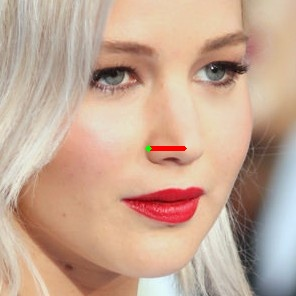
\includegraphics[width=0.675\linewidth]{img/chapter4_analysis/headPose.jpeg}
		\caption{Head pose estimation on close-up of face}
	\end{subfigure}%
	\hspace{\fill} 
	\begin{subfigure}[b]{.5\textwidth}
		\centering
		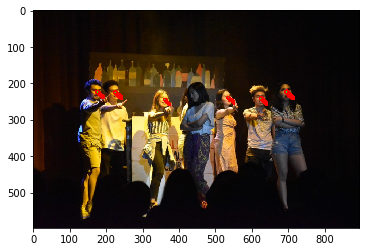
\includegraphics[width=1.0\linewidth]{img/chapter4_analysis/deepgazeWhole.png}
		\caption{Estimation on people at a distance}
	\end{subfigure}
	\vspace{-2\baselineskip}
	\begin{center}
		\caption{DeepGaze head pose estimator}
		\label{fig:deepGaze}
	\end{center}
	\vspace{-2\baselineskip}
\end{figure}

\paragraph{Reasons for removal} We noticed from our research that the head pose estimation was not very accurate, as can be seen in Figure \ref{fig:deepGaze}. A close up image of a face still returns an inaccurate estimation of the head pose. For smaller faces with multiple detections, the head pose estimation was not performed in real-time and also produced inaccurate estimations. Finally, as we will explain in the implementation section, the quality of the images received from the Hololens was too low, and as such, facial landmark detectors required for head pose estimation were unable to detect the keypoints.

\section{Hololens Unity Application}
The Microsoft Hololens is a key component of this project since it acts as the main input, visualization and mapping device. To begin, we utilize the world-facing camera, which sees what the PWU is looking at as the input to the HDD system. Further along the processing pipeline, the Hololens Unity application receives the image co-ordinates of human detections and respective directions to build up a map of the objects in the surroundings. The application manages the holograms, keeping track of the world co-ordinates of the objects, which it sends to ARTA for the reactive control of the wheelchair.
This section covers how the system was designed so that it could be used in conjuction with other ROS nodes despite being a Unity application. It also describes the approach used to develop a front-camera stream, as well as a high level description of the modules responsible for the world mapping and hologram visualization.

\subsection{ROS Node}
Both ARTA and the HDD are implemented on the Robotic Operating System as ROS nodes, and communicate with their sub-nodes using ROS messages across topics. As explained in Section \ref{sec:systemComms}, we view each of the three sub-systems as individual ROS nodes. However, the Hololens does not natively support ROS.

\begin{figure}[ht!]
	\centering
	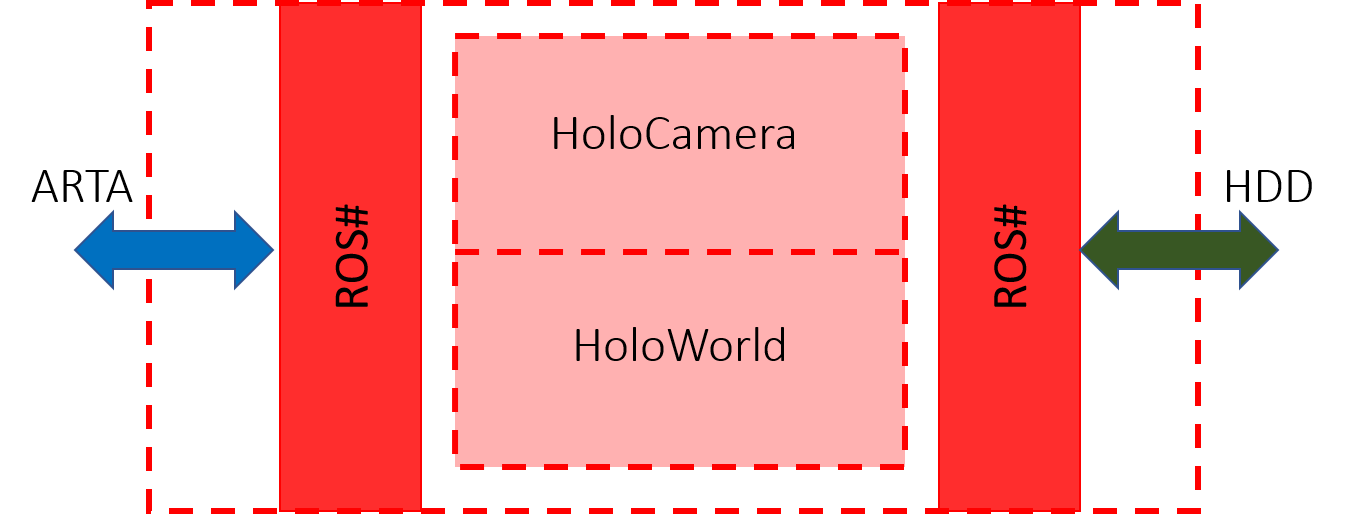
\includegraphics[width=0.8\linewidth]{img/chapter4_analysis/holoROSSharpWrapper.png}
	\caption{ROS\# acts as a ROS wrapper around the Unity application, allowing for seamless communication with other ROS nodes}
	\label{fig:holoROSWrapper}
	\vspace{-1\baselineskip}
\end{figure}

\paragraph{} Since ROS is unable to be run on UWP, we had to use the \textbf{ROS\#} library implemented by Siemens. This allows Unity/UWP applications to send and receive data in the form of ROS messages across topics. Figure \ref{fig:holoROSWrapper} shows how the Unity application is viewed from other ROS nodes as just another node which it can communicate with using topics. The full implementation details of the ROS wrapping are covered later in this report. 

\subsection{HoloCamera}
We begin the Unity application analysis by starting at the beginning of the system pipeline. The HoloCamera is the main visual input to the whole system, prompting the need for a video camera stream to be developed. Previous work done in the PRL have used stationary images taken with the Hololens, but the process of streaming live video from the front camera is a new direction of development. Due to the importance of this step, we spent time researching methods of video streaming to an external computer.

\subsubsection{Video Streaming Choices} \label{sec:videoStreaming}

\paragraph{Windows Device Portal} Microsoft provides a portal to access the Hololens device configuration from a web browser. From the portal, we can manage the connection, control what applications are running and most importantly, access a video stream of the front-facing camera. However, after some testing, we realized that there is a delay of 1-2 seconds between the camera and the video rendered on the computer, making it unsuitable for this project.

\paragraph{Microsoft HoloLensForCV} Another option that was explored was the computer vision development tools released by Microsoft for the Hololens. This library provides developer access to the live camera stream, as well as the raw sensor data, such as the depth and IMU. This would have been the ideal video streaming choice. However, at the beginning of the project, we were not so experienced with developing UWP applications in C\#. Furthermore, it proved difficult to stream the sensor and video streams from a UWP device to a Linux machine, since Windows and Linux have different data formats and standards.

\paragraph{Unity Camera Stream} From our research, we found the \textbf{Vulcan Technologies Hololens Camera Stream} Unity addon library. The community support for Unity development on the Hololens is immense, with various libraries such as the Mixed Reality Toolkit (MRTK) and many other Hololens specific tools. Furthermore, the 3D world modelling and spatial mapping capabilities available in Unity extend the capabilities of an augmented reality system. It abstracts away the complexities of the raw Hololens sensor data, reducing the time to market of applications. Finally, previous work in the PRL involving the Hololens have relied on Unity, making it an ideal choice for this project.

\subsubsection{Module Description}
The HoloCamera module is responsible for accessing the front-camera of the Hololens, compressing the raw image data into a JPEG format and streaming the video frames over the network. The application produces a ROS Compressed Image message that is sent to the HDD for object detection. We provide a complete explanation of the process in the implementation part of this report.

\subsection{HoloWorld}
The goal of this project was to develop an augmented reality system that will assist PWU in navigation by providing visual cues of people in the surroundings. Unity applications have the ability to place holograms in the users surroundings, and render them on the Hololens screen for the user to see. While the majority of the object detection and inference is done on an external computer, the Unity application on the Hololens is used to convert the image co-ordinates of objects into their 3D position in the world. Furthermore, the map of the surroundings is used by the reactive control component of ARTA to avoid collisions with the detected object, making the HoloWorld module a key component of the overall system.

\subsubsection{World Manager}
Since the Hololens is the intermediary, the World Manager sub-module is responsible for managing all the ROS topics between the Hololens, the HDD system and ARTA. The module receives the image co-ordinates from the HDD system and projects the detected points into the world frame. This returns a set of world co-ordinates which we can assign holographic visualizations and map in the Unity world surrounding the Hololens.

\subsubsection{ARTA Alignment} 
With most visual SLAM implementations, the camera attached to the mobile robot is fixed to the robots frame. This simplifies the conversion of the image co-ordiates to the robot frame, and then to the world frame. However, when a PWU wears the Hololens, the front-camera has the ability to move in 6 degrees of freedom. Most importantly, the PWU can turn their head to look left and right. This brings up the issue of not knowing whether a detected object is actually infront of the powered wheelchair, or if the PWU is looking at an object to the side. 

\begin{figure}[ht!]
	\centering
	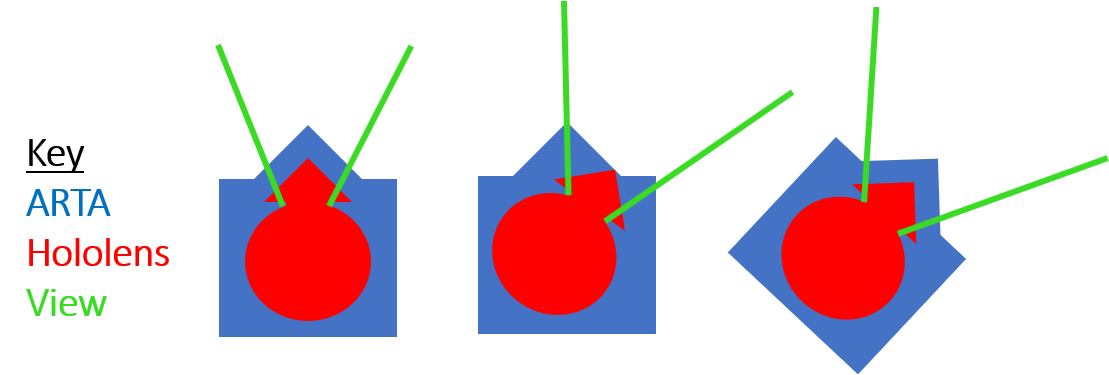
\includegraphics[width=0.9\linewidth]{img/chapter4_analysis/holoArtaAligned.png}
	\caption{We need a way of knowing if a detected object is infront of the wheelchair, or if the PWU is looking to the side. }
	\label{fig:holoArtaAlignment}
\end{figure}

\paragraph{}We visualize this problem in Figure \ref{fig:holoArtaAlignment}. When the Hololens camera and wheelchair frames are aligned, it is easy to tell if an object is in the path of the wheelchair. For the reactive control component of ARTA, we need to know if an object is in ARTAs current trajectory to determine if a collision will occur. As such, This module is responsible for discerning between people being in front of the wheelchair or to the side. 

\section{ARTA}
The Personal Robotics Lab (PRL) at Imperial College London have built and developed an original smart powered wheelchair known as the Assitive Robotic Transport for Adults (ARTA). The wheelchair was designed to assist adults with mobility issues, and is frequently used in the PRL as a research topic in conjunction with exotic control interfaces such as the Hololens \cite{Zolotas2018, Chacon-Quesada}.

\subsection{Breakdown}

To Write

\chapter{Implementation}
This chapter is concerned with the implementation details of the individidual components introduced in Chapter \ref{chapter:4}. This includes the development of the Unity application responsible for producing the front-facing camera video stream and displaying the visual cues, the development of the human detection and direction system, as well as the reactive control systems implemented on ARTA. Previous work in the PRL had utilized the Hololens camera to capture images that were then processed on an external computer, but where this project differs is that a video stream is required to perform real-time object detection. As such, a large amount of time was spent at the very beginning of the project trying to produce a video stream, since the whole project depended on this form of visual input.

\begin{figure}[ht]
	\centering
	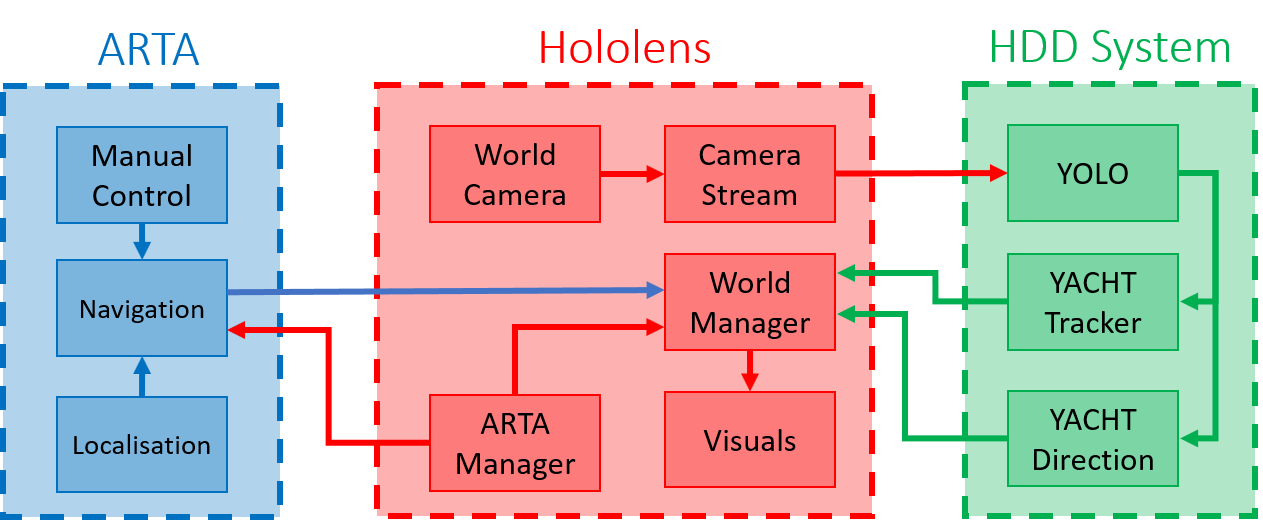
\includegraphics[width=1.0\linewidth]{img/chapter5_implementation/detailedSystemDiagram.png}
	\caption{System diagram detailing individual components}
	\label{fig:detailedHL}
\end{figure}

Figure \ref{fig:detailedHL} is a more detailed diagram of the high level system digram presented in Figure \ref{fig:simplifiedHL}. We show the communication between the three seperate devices, and how each node can be broken down into smaller nodes running specific computations. For the rest of this report, we represent the ARTA, Hololens and HDD system components with the colours blue, red and green respectively.

%\section{Hololens Video Camera Stream}
%For this project to begin, it was absolutely essential to stream the front-facing camera on the Hololens to another PC. Once it had been proven that this was possible, work on the rest of the project could begin. As such, the first month of the project was spent comparing different camera streaming methods. As mentioned in Section \ref{sec:videoStreaming}, we briefly spent some time attempting to use the HoloLensForCV library from Microsoft. However, after speaking with several members of the PRL, it was decided the best method would be to use the Unity application approach as a base.

\section{Human Detection \& Direction System}
In order to determine the direction people are walking in, it is necessary for the system to be able to detect humans. Only after detection is it possible to discern the motion of individuals, which can be achieved through object tracking and body pose estimation. Figure \ref{fig:detailedHDD} shows the breakdown of the HDD node into components responsible for these two tasks. This section is concerned with the implementation of the methods needed to perform the direction prediction, as well as how the system communicates between its nodes. 

\begin{figure}[ht]
	\centering
	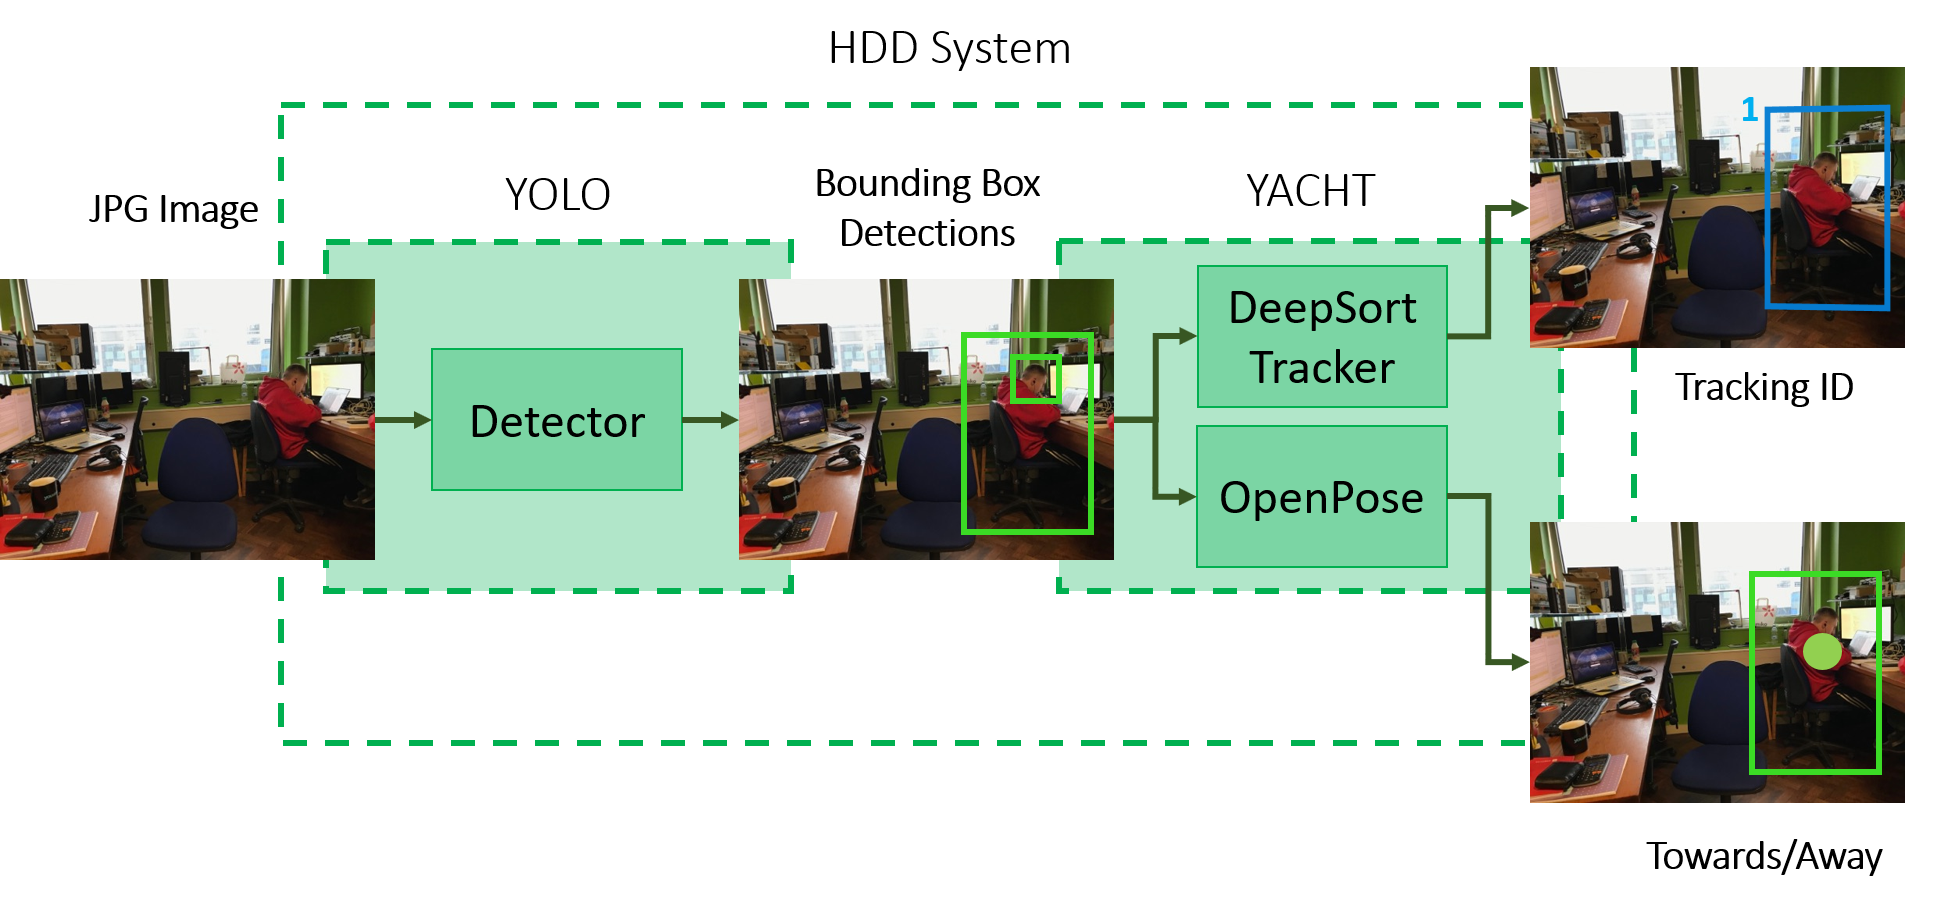
\includegraphics[width=1.0\linewidth]{img/chapter5_implementation/hddSystemDiagram.png}
	\caption{Individual nodes in HDD System}
	\label{fig:detailedHDD}
\end{figure}

We begin this section by listing the hardware requirements for the system. Due to the nature of the HDD, and its reliance on modern deep learning techniques, access to a modern GPU is essential. We refrain from trying to explain the step-by-step process to setup the hardware and software, and instead point the reader in the direction of an article\footnote{https://link.medium.com/xQ5w2FMXoX} which covers this topic.

\subsection{Hardware \& Software Dependencies}

\subsubsection{Hardware}
We implemented the HDD system on a desktop computer connected to the Imperial College network. Due to the real-time computer vision requirements of this project, the computer was chosen due to the GTX 1050Ti GPU with 4GB video RAM available on the system. The computer was also equipped with an Intel i7-2600 CPU and 8GB DDR3 RAM.

\subsubsection{Software}
We have refrained from posting all Python dependencies for the project and only mention the key ones. A complete listing is available in the appendix. The following software dependencies are required to run this project:
\begin{itemize}
	\item Ubuntu 16.04
	\item Python 2.7
	\item OpenCV 3.0
	\item ROS Kinetic
\end{itemize}

Due to the deep learning component of the project, the following software dependencies are essential:
\begin{itemize}
	\item Nvidia Graphics Drivers 
	\item CUDA 8.0 Toolkit
	\item cuDNN 6.0
	\item Darknet
	\item Tensorflow-GPU
	\item Caffe
\end{itemize}

\subsection{YOLO Object Detector}
As mentioned in Section \ref{sec:yolo}, we chose to use the YOLOv3 Tiny architecture and trained it on the CrowdHuman dataset. We begin this section by introducing the reader to \textbf{Darknet}, the neural network framework YOLO is implemented on, and how we integrated it into ROS. We also briefly explain how the network detects objects, and compare YOLOv3-tiny with the more memory intensive YOLOv3. We then guide the reader through the training process, and the analysis we did to validate the human detection improvements compared to pre-trained models.

\subsubsection{Darknet}
Darknet\footnote{https://pjreddie.com/darknet/} is an open source neural network framework written in C and CUDA which supports both CPU and GPU computation \cite{darknet13}. The source code for the framework is freely available on Github, and it can be used to train different neural network architectures in a manner similar to more conventional deep learning frameworks such as Tensorflow or Caffe.

\subsubsection{Darknet in ROS}
By definition, ROS is language-independent, although at the time of writing, three main libraries have been defined for ROS, making it possible to program ROS in Python, Lisp or C++. On the other hand, Darknet is implemented in C, due to the speed of compiled low-level languages in conjunction with CUDA. However, the Darknet framework is compiled into \textit{Shared Object (.so)} file, which is analogous to a Windows DLL. As such, it becomes possible to access the framework by writing wrappers around the compiled library file.

\paragraph{}Darknet has basic Python wrappers around the compiled library which convert Python datatypes into C and vice versa. However, the original wrappers for detection are written to run on images that are saved on disk. Darknet converts the saved images into a C data structure \code{IMAGE} and performs the detections. To integrate the framework into ROS, the node must be able to receive data from image topics with \code{CompressedImage} or raw \code{Image} messages.

\paragraph{}In ROS Python, the JPG or PNG images received from the \code{CompressedImage} message can be converted to numpy arrays which store the RGB values, without the need to be saved on disk. As such, we wrote Python wrappers for Darknet that allow the framework to support images in the form of numpy arrays as well as images saved on disk. The following listing defines the \code{IMAGE} data structure, and the conversion of an image numpy array to the Darknet format: \\



\begin{lstlisting}[language=Python, caption={Darknet IMAGE Python wrappers}]
# IMAGE: a C data structure used by Darknet
class IMAGE(Structure): 
	_fields_ = [("w", c_int),
				("h", c_int),
				("c", c_int),
				("data", POINTER(c_float))]
				
# Converts numpy array to Darknet IMAGE type
def nparray_to_image(img): 
	data = img.ctypes.data_as(POINTER(c_ubyte))
	image = ndarray_image(data, img.ctypes.shape, img.ctypes.strides)

	return image
\end{lstlisting}

Further Python wrappers were written for the detection and return of the image bounding box co-ordinates. We also created ROS messages for the bounding box detections, which allows the Darknet YOLO node to communicate with other nodes in the HDD system. The full code listing can be found in the Appendix \footnote{https://github.com/alaksana96/darknet-crowdhuman}\footnote{https://github.com/alaksana96/fyp\_yolo}.

\subsubsection{YOLO Detection Algorithm}
As researched in Section \ref{sec:backYOLO}, the algorithm divides an input image into an $S\times S$ grid. Each grid cell can predict one object, and a cell can predict a fixed number of bounding boxes $B$, which we visualize in Figure \ref{fig:yoloViz}. The predicted bounding box is chosen from the set of $B$ boxes with the highest box confidence score, which is a measure of how likely the box contains an object and how accurate the boundry box is. It also predicts the conditional class probability, which is the probability a detected object belongs to a certain class. 

\begin{figure}[ht]
	\begin{subfigure}[b]{.45\textwidth}
		\centering
		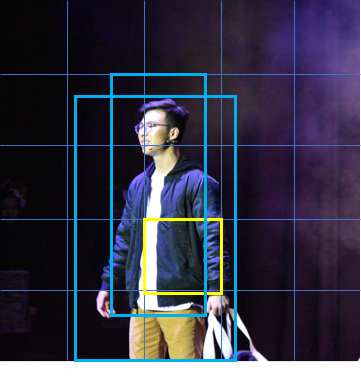
\includegraphics[width=1.0\linewidth]{img/chapter5_implementation/yoloAlgo1.png}
		\caption{A grid cell can make $B$ predictions, in this example $B=2$}
	\end{subfigure}%
	\hspace{\fill} 
	\begin{subfigure}[b]{.45\textwidth}
		\centering
		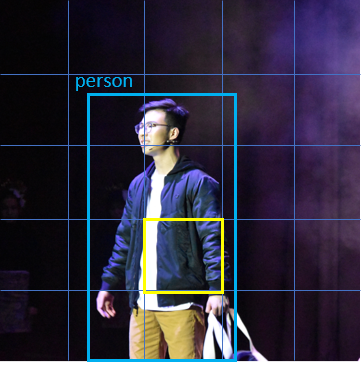
\includegraphics[width=1.0\linewidth]{img/chapter5_implementation/yoloAlgo.png}
		\caption{The bounding box with higher box confidence score is used}
	\end{subfigure}
	\vspace{-1\baselineskip}
	\begin{center}
		\caption{Visualization of YOLO person detection}
		\label{fig:yoloViz}
	\end{center}
	\vspace{-2\baselineskip}
\end{figure}

\subsubsection{YOLOv3 Tiny vs YOLOv3}
While testing out the different models, we noticed that the YOLOv3 model was consistently crashing and causing segmentation faults. On further investigation, we noticed that this was due to the network using up all 4GB of video memory available on the GPU. In comparison to its predecessors YOLO and YOLOv2, YOLOv3 is a much larger network which has 106 fully convolutional layers. Although it is far more accurate at predicting bounding boxes, it reduces the framerates that can be achieved on video. As such, we decided to use YOLOv3 Tiny, a shallower variant of the network that is suitable for real-time image detection. Although the tiny version is not as accurate, it is much lighter on memory, using less than 1GB video RAM, making it a suitable choice for this project.

\subsubsection{Training YOLOv3 Tiny}
\paragraph{CrowdHuman} The CrowdHuman dataset \cite{Shao} is a benchmark dataset to better evaluate detectors in crowd scenarios. The most important features of the dataset are the size, quality of the annotations and the diversity. Each image contains multiple people with varying degrees of occlusion, which allows for object detectors to better learn the representation of obscured people. 

\begin{figure}[ht]
	\centering
	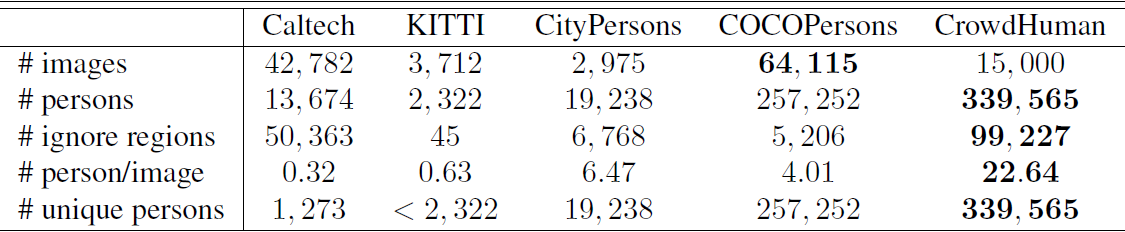
\includegraphics[width=0.8\linewidth]{img/chapter5_implementation/crowdHumanStats.png}
	\caption{A comparison of CrowdHuman to other person image datasets \cite{Shao}}
	\label{fig:crowdHumanStats}
\end{figure}

As can be seen from Figure \ref{fig:crowdHumanStats}, the dataset contains far more unique identities. By examining the dataset, we can see that it contains people in a wide array of situations, at varying distances with different body poses.

\paragraph{Annotations} The CrowdHuman dataset provides its annotations in the \code{.odtg} format, which is a variant of JSON. Each line in the annotation file corresponds to a JSON containing the image ID and the bounding boxes. The annotations include boxes for the \textit{visible box}, \textit{full body box} and \textit{head box}. For the purposes of this training, we chose to use the full body and head boxes only. We wanted the detector be able to learn to predict occluded individuals, and we also wanted to experiment with head pose estimation. Each bounding box is annotated as below, where \code{x,y} is the top-left corner of the bounding box. The \code{width} and \code{height} are also given in image co-ordinate pixels.

\paragraph{}\code{[x, y, width, height]}  

\paragraph{}On the other hand, to train YOLO on Darknet, the annotations must be given in a completely different format. The Darknet annotation format is as such:

\paragraph{}\code{<object-class> <x> <y> <width> <height>}

\paragraph{}Since Darknet accepts images of any size, it works with image units which are scaled relative to the size of the image. As such, all the values for the bounding boxes are between $0$ and $1$. Furthermore, the \code{x, y} values in the annotation are measured from the centre of the bounding box.  

\paragraph{Converting Annotations} To use the CrowdHuman images as a training set for the YOLOv3-tiny model, we had to write several scripts that converted the annotations to the Darknet format. We have included these scripts in the Appendix should the reader wish to convert the dataset themselves\footnote{https://github.com/alaksana96/darknet-crowdhuman/blob/master/README.md}.

\paragraph{Training Parameters} Before training, we set up the model configuration file to learn 2 classes, head and body, as well as to use batches of 32 divided into subdivision of 8 images. This limits the number of images loaded into memory at once to 8, to prevent running out of GPU memory. We also reduce the size of the training images to $416\times 416$ pixels, to further reduce the GPU usage. \\

\begin{lstlisting}[language=Mymatlab,caption={Training parameters}]
	batch=32 %Training parameters for YOLO Tiny
	subdivisions=8
	width=416
	height=416
	channels=3
	momentum=0.9
	decay=0.0005
\end{lstlisting}

These optimizations were done in order to maximize the amount of GPU memory used for training, without a sudden surge in usage causing a segmentation fault. Resizing the input training images allows the algorithm to divide the image into a $S\times S$ grid. Generally, the larger the height and width, the better the predictions, since the image can be divided into more grid cells. This is a trade-off we had to make in order to be able to train the network on a mid-range GPU.

\paragraph{Training Process} We left the model to train overnight, creating backups of the weights every 1000 iterations. The following day, after reaching 30,000 iterations, we decided to stop training the network. The average loss error and total loss had stopped decreasing for several hours, and was hovering around $29.134$. We reasoned that the network had reached a minima, and further training would be redundant, since it would overfit the dataset. The final weights are available in the file \code{yolov3-tiny-crowdhuman.backup} .

\subsubsection{Evaluating Trained Model}
\paragraph{Hololens Videos} As mentioned in Section \ref{sec:backYOLO}, we recorded several test videos using the Microsofto Hololens. These videos were capture in various locations on the Imperial College campus. A common area where lots of people frequent is the Sherfield walkway. As seen in Figure \ref{fig:yoloSherfield}, this was an ideal place to capture a video since it features a lot of people walking around in different directions. We captured several more videos outside the EEE building and inside the 5th floor ICRS lab. 

\begin{figure}[ht]
	\centering
	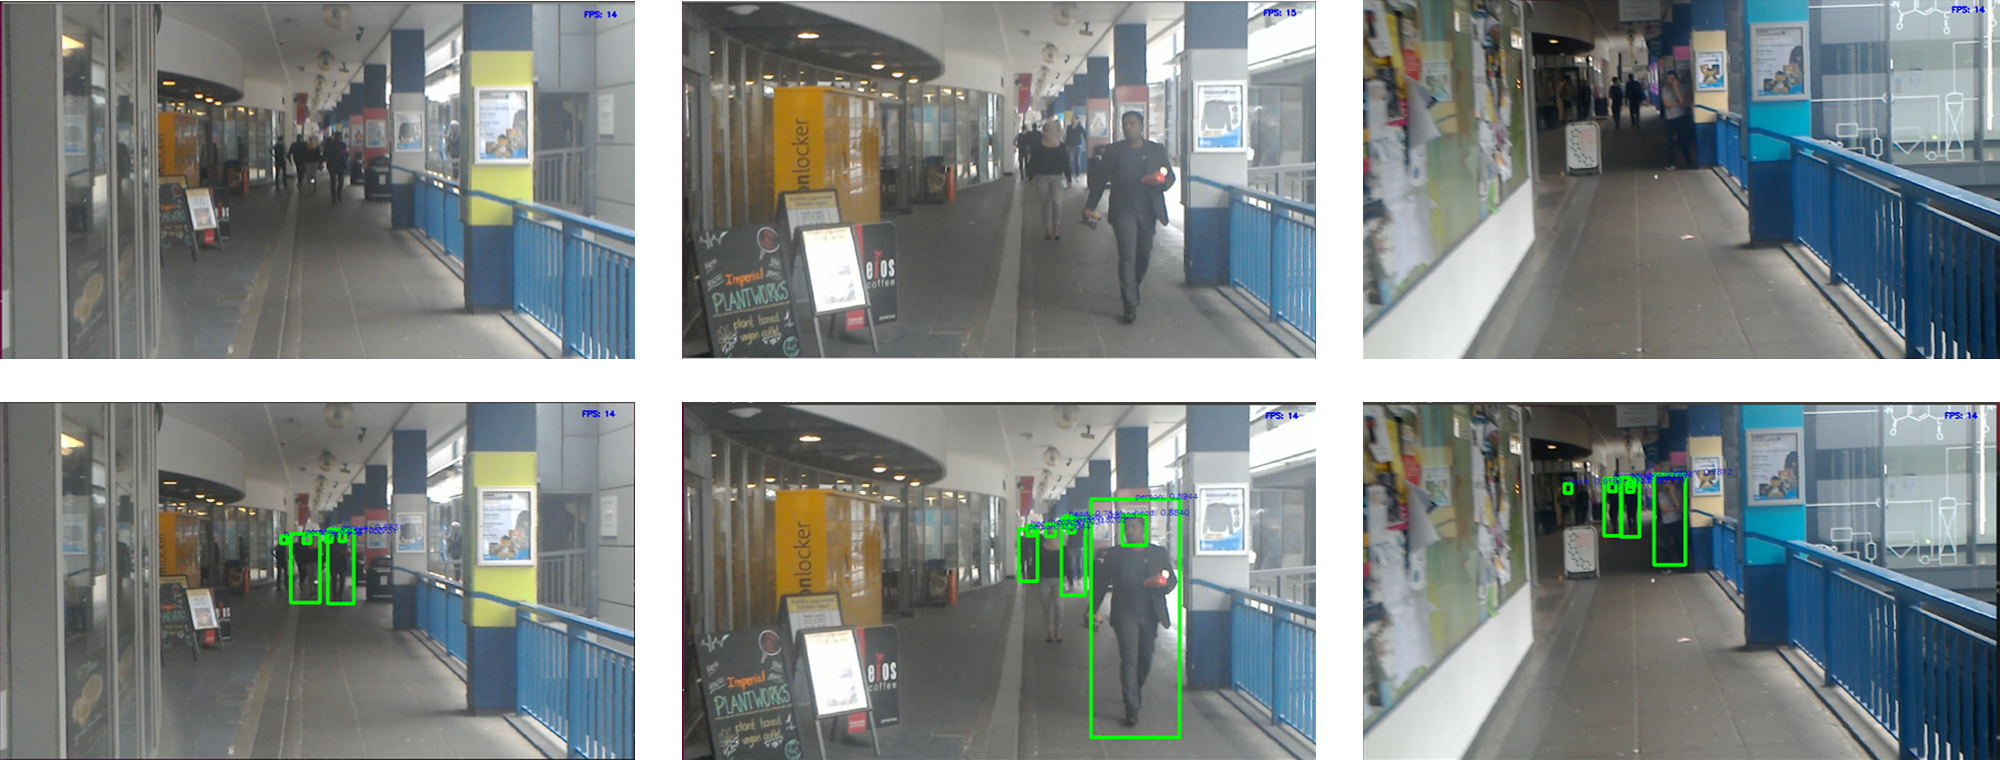
\includegraphics[width=0.95\linewidth]{img/chapter5_implementation/yoloWalkwayMultiple.png}
	\caption{Evaluating the model on Sherfield Walkway test video}
	\label{fig:yoloSherfield}
\end{figure}

\paragraph{} The videos from the Hololens were captured whilst a person was walking with the device, to best emulate a PWU in a wheelchair navigating through populated areas. We noticed an improvement in the number and accuracy of the detected bounding boxes compared with the pre-trained COCO models provided by Darknet. The most significant improvement to the model was the ability to detect objects at different ranges, as shown in Figure \ref{fig:yoloRange}. 

\begin{figure}[ht]
	\centering
	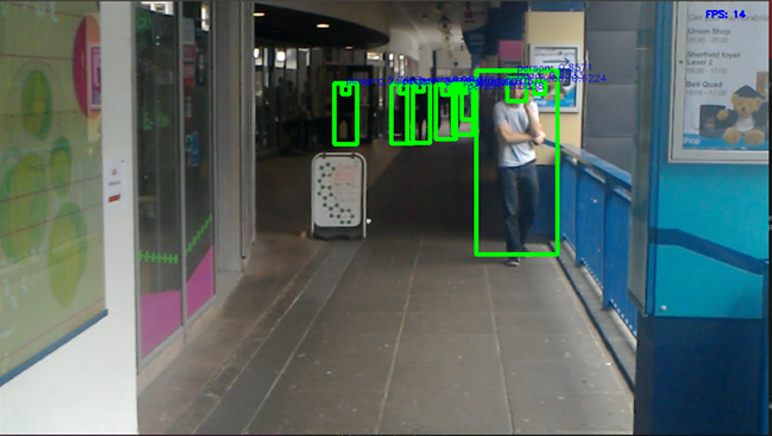
\includegraphics[width=0.8\linewidth]{img/chapter5_implementation/yoloWalkway.png}
	\caption{Trained model detects people and heads at different ranges}
	\label{fig:yoloRange}
\end{figure}

\subsubsection{ROS Node} \label{sec:nodeYOLO}
The Python wrappers for Darknet allow us to access the detection and image conversion functionality of the framework. To fully integrate the framework as a ROS node, we must follow the standard ROS procedures for creating a new ROS package. As such, we have created a package\footnote{https://github.com/alaksana96/fyp\_yolo} that runs Darknet and YOLO that can be downloaded and run seamlessly with ROS.

\paragraph{ROS Topics} The ROS node subscribes to the \code{/image\_transport/compressed} and expects to receive images in the compressed JPG format. This is because the Hololens captures video frames and encodes it to reduce the usage on the network bandwidth. These images are converted to numpy arrays which are further converted to Darknet \code{IMAGE} types for detection. 

\paragraph{} Darknet produces bounding box co-ordinates and class probabilities for each detection in an image. For every received frame, the node publishes the original image and a list of associated bounding boxes. The bounding box message contains the following information: \\

\begin{lstlisting}[language=Mymatlab,caption={BoundingBox.msg},label={bbmsg}]
string Class
float64 probability
int64 xmin % Top Left Corner
int64 ymin
int64 xmax % Bottom Right Corner
int64 ymax
\end{lstlisting}

\subsection{YACHT Package}
The major contribution of this project is in the form of the Yet Another Crowd Human Tracker package for ROS. This package utilizes the Deep SORT algorithm and OpenPose body pose estimation framework to attempt to determine the direction of individuals.


\paragraph{ROS Communication} As seen in Section \ref{sec:nodeYOLO}, the YOLO object detector node publishes a topic which contains the image and associated bounding boxes. Figure \ref{fig:detailedHL} shows that both YACHT nodes subscribe to the same output topic. The reason we decided to include the original image in the message and not just the bounding boxes is so that we can be sure the bounding boxes were detected for that frame, without having to subscribe to two seperate topics and comparing timestamps on individiual messages.

\subsection{YACHT: Tracker}
As explained in Section \ref{sec:YACHT}, the YACHT tracker depends on the Deep SORT algorithm \cite{Wojke2018}. Using the detections produced by the YOLO node, we assign IDs and match them across video frames to produce a track. These tracking IDs are then sent to the HoloLens for visualizaiton.


\subsubsection{Deep SORT} 

\paragraph{Modifications} We have modified\footnote{https://github.com/alaksana96/deep\_sort} Nicolai Wojke's original implementation of Deep SORT to run on Tensorflow-GPU. In the original, as the number of detections increased, so does the delay in tracking. This issue is more prevalent when tested on the MOT dataset, which has a large number of objects in each frame. Figure \ref{fig:deepSortCPU} visualizes the delay on the MOT16-06 video. We can see that the algorithm is operating at a very low FPS, causing it to be delayed in time. 

\begin{figure}[ht]
	\begin{subfigure}[b]{.45\textwidth}
		\centering
		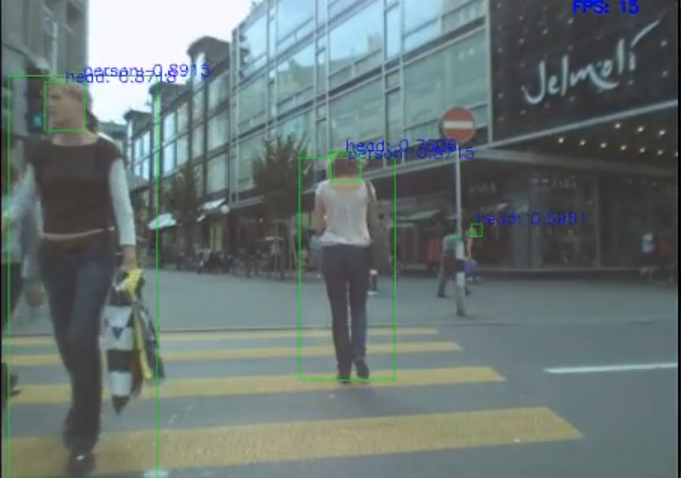
\includegraphics[width=1.0\linewidth]{img/chapter5_implementation/deepSortCPU.png}
		\caption{Output of YOLO. The image frame and bounding boxes are fed to Deep SORT}
	\end{subfigure}%
	\hspace{\fill} 
	\begin{subfigure}[b]{.45\textwidth}
		\centering
		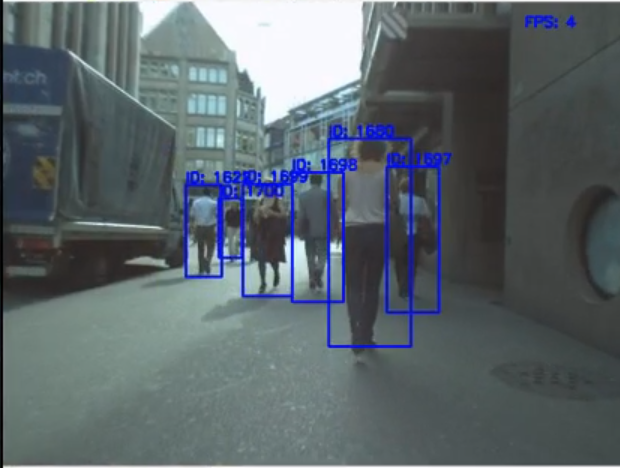
\includegraphics[width=0.935\linewidth]{img/chapter5_implementation/deepSortCPU1.png}
		\caption{Deep SORT is several frames behind since it runs at 4 FPS}
	\end{subfigure}
	\vspace{-1\baselineskip}
	\begin{center}
		\caption{Visualization of delay on CPU bound Deep SORT}
		\label{fig:deepSortCPU}
	\end{center}
\end{figure}


\paragraph{Deep Association Metric} Through code profiling, we noticed that the program was spending a lot of time in the generation of feature vectors. Upon inspection, we noticed that this process was run on a CPU bound version of Tensorflow. The \code{ImageEncoder} class uses a pre-trained deep network that generates the feature vectors for each bounding box. By using Tensorflow-gpu, we were able to run the network on system GPU, removing the delay. \\

\begin{lstlisting}[language=Python, caption={Deep SORT Tensorflow GPU modifications}]
class ImageEncoder(object):

	def __init__(self, checkpoint_filename, input_name="images",
				 output_name="features"):
				 
        # Tensorflow-GPU
        gpu_options = tf.GPUOptions(per_process_gpu_memory_fraction = 0.2)
        self.session = tf.Session(config=tf.ConfigProto(gpu_options=gpu_options))
\end{lstlisting}

%The tracker crops the image and generates feature vectors for the detection. The vectors are then compared with the history of feature vectors associated with each tracker.

\paragraph{Trackers \& Tracking} For each detection, we generate a feature vector using the image pixels within the bounding box. A matching cascade with Nearest Neighbour metric is used to best match the detection with existing confirmed tracks. Some detections will not get matched since the distance to confirmed tracks is above the \code{matching\ threshold}. The algorithm then attempts to match the detections to unconfirmed tracks using a simple Intersection-over-Union metric. These are newly created tracks that have existed for less than the last $n$ frames. If the detection is still unmatched, the algorithm creates a new tracker for the detection and adds it to the pool of unconfirmed tracks.

\begin{figure}[ht]
	\centering
	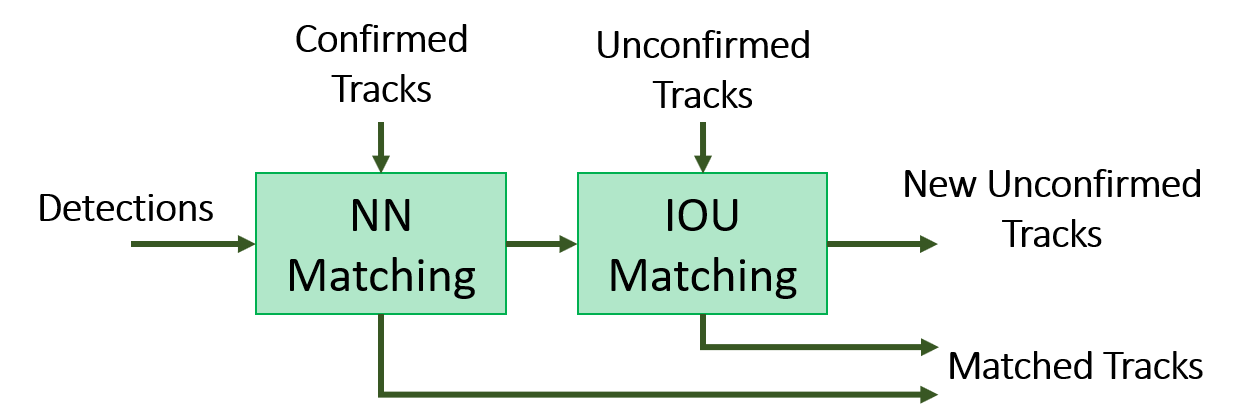
\includegraphics[width=0.8\linewidth]{img/chapter5_implementation/deepSortMatching.png}
	\caption{Deep SORT matching visualized}
	\label{fig:deepSortMatch}
\end{figure}

Any pre-existing tracks which are not matched are checked. If the number of frames since the previous match is greater than the \code{max\_age} parameter, the track is considered dead and is deleted. This is done so as to prevent the number of tracks from growing unboundedly. A Kalman filter is used to update the bounding box states of each track, as well as the time since the last update.
 
\subsubsection{Linear Extrapolation}
We experimented with linear extrapolation across frames as a way of infering the direction travelled by the detection. As the project progressed, we encountered issues with this method, as explained in Section \ref{sec:objecTrackingDirection}. By searching for alternative methods, it was found that the depth camera on the Hololens can determine the distance between the PWU and an object relatively accurately. As such, we abandoned the pure computer vision approach in favour of using the Hololens.

\subsubsection{ROS Topic} The decision to use the Hololens depth cameras as a way of determining distance prompted the need for ROS messages to be sent to the device. As seen in Figure \ref{fig:detailedHDD}, the  tracker node publishes the bounding box and tracker ID to the Hololens. The \code{BoundingBox} data structure is defined in Listing \ref{bbmsg}, and is the same bounding boxes generated by the YOLO detector.

\begin{lstlisting}[language=Mymatlab,caption={BoundingBoxID.msg}]
BoundingBox boundingBox
int64 id
\end{lstlisting}

\subsection{YACHT: Direction}
The second node in the YACHT package is the direction node, which uses the OpenPose framework to determine if a person is facing the camera or not. Earlier in Section \ref{des:YACHTBody}, we outlined the problem of not being able to determine the distance to an object with a regular pinhole camera model. We initally wanted to be able to determine the distance using only a video stream and computer vision techniques. However, we quickly realized that this was beyond the scope of the project, and decided to use the depth cameras on the Hololens.

\paragraph{} This section outlines the installation and setup of the OpenPose network \cite{Shao}. We also explain how we use the keypoint detections to determine whether an individual is facing the PWU or not. Furthermore, we also explain how the bottom-up approach of OpenPose differs from the top-down approach that may have been more suitable, and the reasons for our implementation choices.

\subsubsection{OpenPose}
OpenPose is developed and maintained by the Carnegie Mellon University Perceptual Computing Lab. The implementation is made available on Github\footnote{https://github.com/CMU-Perceptual-Computing-Lab/openpose} to encourage body pose estimation research.

\paragraph{Installation \& Setup} The OpenPose library runs on a modified version of the convolutional neural network framework Caffe \cite{Jia}. The library is well documented, and provides its own instructions on how to setup the library. We direct the reader to the OpenPose Github repository if they wish to install the library themselves.

\paragraph{Model} As stated in Section \ref{des:body_25}, we use the \code{BODY\_25} keypoint estimation model for this project. The documentation states that this model is the fastest when it comes to real-time application, compared to the \code{MPI\_4} or \code{COCO} models. We also reduce the network resolution to $176\times 176$ to reduce the GPU usage and speed up the keypoint estimation. However, this reduces the accuracy of the detections, as discussed in this section.

\subsubsection{KeyPoint Estimation} \label{sec:bottomUp} 
Due to the bottom-up approach used by OpenPose, the network predicts keypoints for individual body parts across the whole image. Through our testing on the MOT dataset, we noticed several points:

\begin{itemize}
	\item The model is good at detecting keypoints of people close to the camera.
	\item People who are smaller and further away are not always detected.
	\item When people are close together or overlap, the keypoint estimation has difficulty differentiating between people.
	\item The more people in the image, the more network slows down and begins to lag behind the source video.
\end{itemize}

\begin{figure}[ht]
	\begin{subfigure}[b]{.32\textwidth}
		\centering
		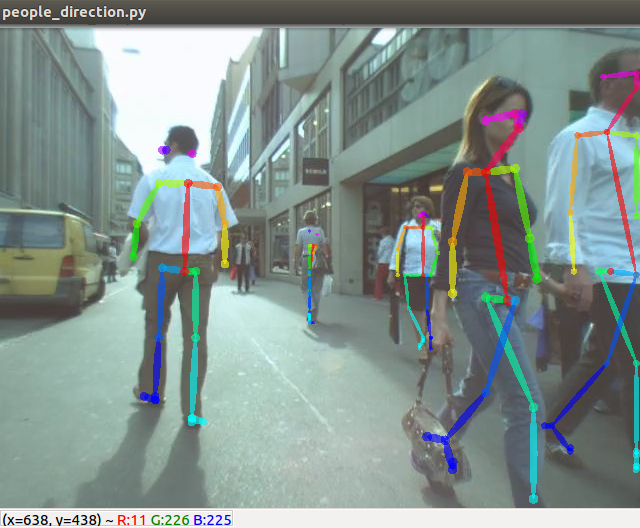
\includegraphics[width=1.0\linewidth]{img/chapter5_implementation/openposeKP.png}
		\caption{People close-up}
	\end{subfigure}%
	\hspace{\fill} 
	\begin{subfigure}[b]{.32\textwidth}
		\centering
		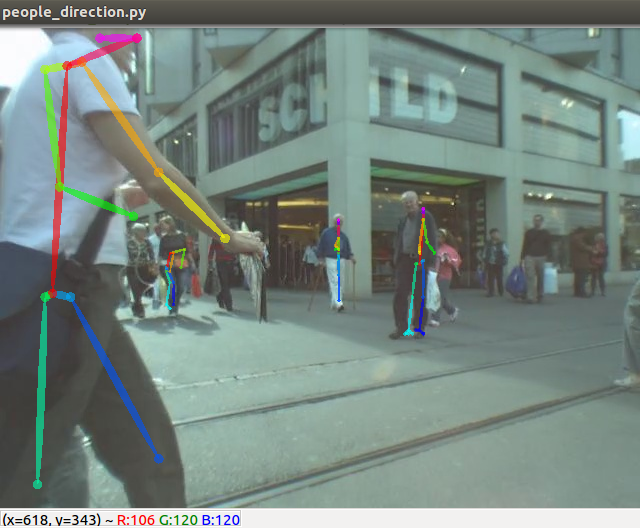
\includegraphics[width=1.0\linewidth]{img/chapter5_implementation/openposeKP1.png}
		\caption{People at different scales}
	\end{subfigure}
	\hspace{\fill} 
	\begin{subfigure}[b]{.32\textwidth}
		\centering
		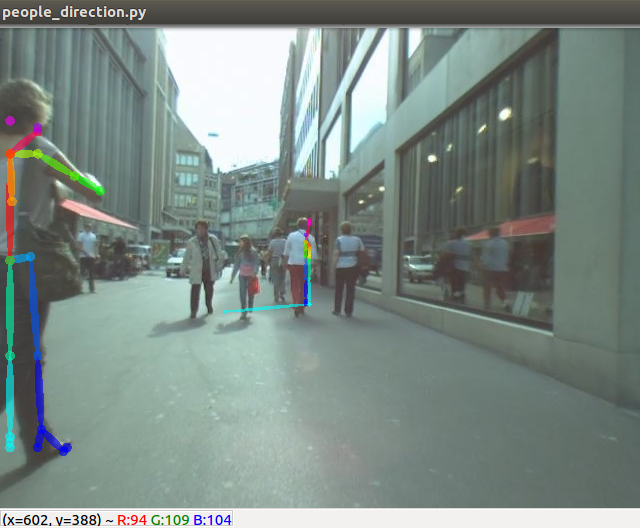
\includegraphics[width=1.0\linewidth]{img/chapter5_implementation/openposeKP2.png}
		\caption{People close together}
	\end{subfigure}
	\vspace{-1\baselineskip}
	\begin{center}
		\caption{Comparison of keypoint estimation at different scales}
		\label{fig:openposeKP}
	\end{center}
		\vspace{-1.5\baselineskip}
\end{figure}

We highlight the issues in Figure \ref{fig:openposeKP}. The reason for the decrease in accuracy on people further away is due to the network resolution being lowered. Using a higher resolution allows us to detect people further away, but the delay between the arrival of the frame and the detection is more than 0.5 seconds. As such, to achieve real-time operation, we chose to use a lower network resolution.

\subsubsection{Defining Direction}
By comparing the relative positions of certain keypoints, we can determine if a person is facing towards the camera or if they are walking away. This information is important, since it will allow for better visualization of where a person is walking, since people tend to walk in the direction they are facing. This also partially solves the direction problem brought up in Section \ref{sec:objecTrackingDirection}.

\begin{figure}[ht]
	\begin{subfigure}[b]{.32\textwidth}
		\centering
		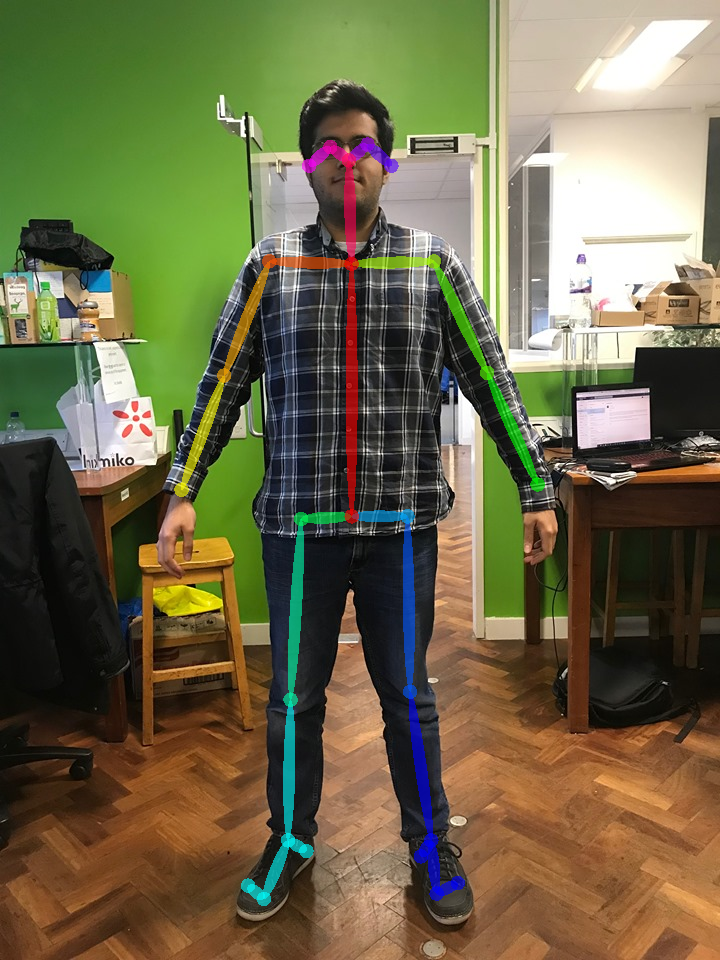
\includegraphics[width=1.0\linewidth]{img/chapter5_implementation/shreyFront.png}
		\caption{Frontal View}
	\end{subfigure}%
	\hspace{\fill} 
	\begin{subfigure}[b]{.32\textwidth}
		\centering
		\includegraphics[width=0.765\linewidth]{img/chapter5_implementation/keypoints_pose_25.png}
		\caption{Keypoint References}
	\end{subfigure}
	\hspace{\fill} 
	\begin{subfigure}[b]{.32\textwidth}
		\centering
		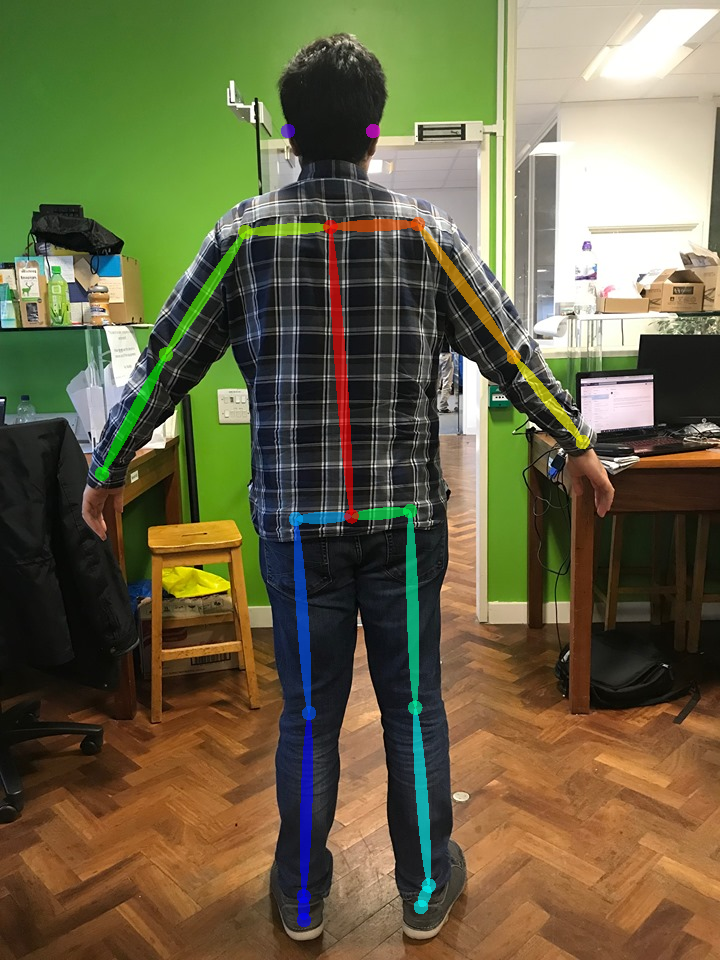
\includegraphics[width=1.0\linewidth]{img/chapter5_implementation/shreyBack.png}
		\caption{Back View}
	\end{subfigure}
	\vspace{-1\baselineskip}
	\begin{center}
		\caption{Body keypoint estimation of different views}
		\label{fig:keypointShrey}
	\end{center}
	\vspace{-2\baselineskip}
\end{figure}

\paragraph{Method} Pixels are measured from the top left corner of the image, with the x-axis extending horizontally to the right and the y-axis extending downwards. Figure \ref{fig:keypointShrey}.b shows the keypoint references for the body. The model is able to differentiate between the left and right limbs on a person. Figure \ref{fig:keypointShrey}.(a,c) show a full frontal and back keypoint detection on a person in the ideal detection position. 

\begin{table}[ht]
	\centering
	\begin{tabular}{|l|l|}
		\hline
		Body Part  & Key Points \\ \hline
		Right Arm  & 2, 3, 4    \\ \hline
		Left Arm   & 5, 6, 7    \\ \hline
		Head/Spine & 0, 1, 8    \\ \hline
	\end{tabular}
	\caption{Significant keypoints for direction}
	\label{tab:keypoints}
\end{table}

We can use the ability to differentiate between the left and right arms to determine if a person is facing the camera. Table \ref{tab:keypoints} presents the keypoints for the relevant bodyparts. If the image co-ordinates of the left shoulder is further along the x-axis than the right shoulder, we can predict the direction as facing towards the camera. From testing, we know this simple method works most of the time. However, problems arise when a person is standing perpendicular to the camera. OpenPose has trouble detecting the torso and predicting the positions of the limbs, and it becomes difficult to decide if they are facing left or right.

\subsubsection{Implementation \& Detection Matching}
As mentioned in Section \ref{sec:bottomUp}, OpenPose uses a bottom-up approach by detecting individual body parts across the whole image. We need to match the OpenPose keypoint predictions with existing bounding boxes from YOLO, since these are assigned track IDs by the tracker node. This is done in Listing \ref{lst:matchDetPose} \\

\begin{lstlisting}[language=Python, caption={Direction and Detection Matching}, label={lst:matchDetPose}]
def matchDetectionAndPose(self, detections, poses):
    for pose in poses:
        # Check torso, right/left shoulder
        torso, rshoulder, lshoulder = pose[1], pose[2], pose[5]

        for bbox in detections:
            if( self.withinBB(bbox, torso[0], torso[1]) or
                self.withinBB(bbox, rshoulder[0], rshoulder[1]) or
                self.withinBB(bbox, lshoulder[0], lshoulder[1])):
   
                if(rshoulder[0] > lshoulder[0]):
                    directionTowardsCamera = False
                else:
                    directionTowardsCamera = True

                publishDetectionDirection() 
                break # Once matched, move onto next pose 
\end{lstlisting}

\subsubsection{}


\subsection{YACHT ROS Communication}


%\section{Hololens Unity Application}
%
%\begin{figure}[ht]
%	\centering
%	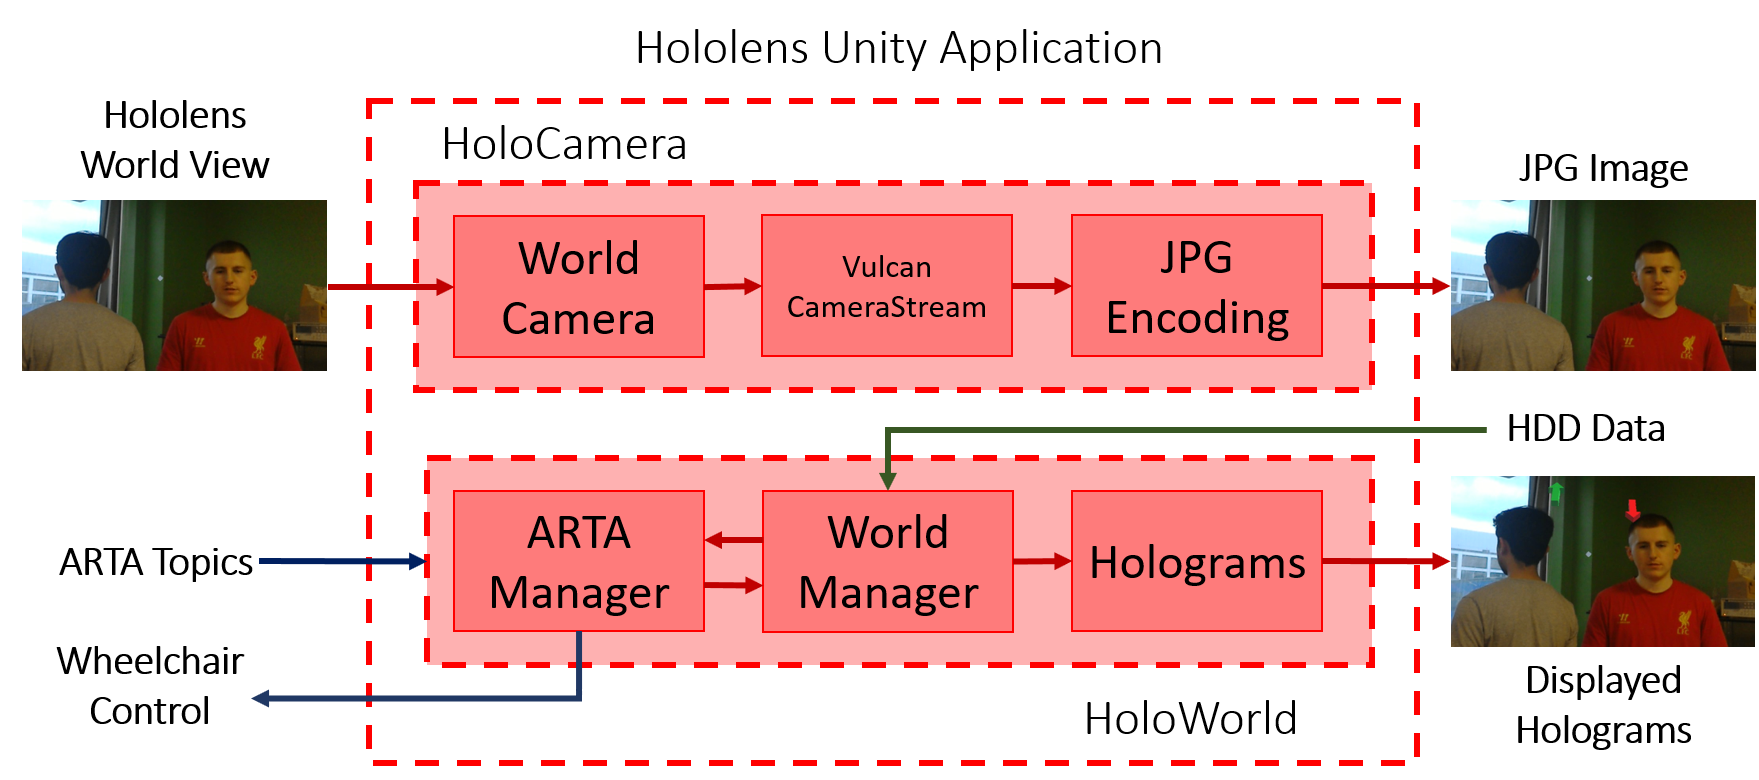
\includegraphics[width=1.0\linewidth]{img/chapter5_implementation/hololensSystemDiagram.png}
%	\caption{Unity application running on the Hololens}
%	\label{fig:detailedHololens}
%\end{figure}


\bibliographystyle{unsrt}
\bibliography{fyp_report.bib}

\end{document}